\documentclass[letterpaper, 10 pt, conference]{ieeeconf}
\IEEEoverridecommandlockouts
\overrideIEEEmargins

\usepackage[utf8]{inputenc}
\usepackage[T1]{fontenc}
\usepackage[english]{babel}
\usepackage{booktabs}
\usepackage{tabularx}
\usepackage{multirow}
\usepackage{listings}
\usepackage{subcaption}
\usepackage{xcolor}
\usepackage{xspace}
\captionsetup{font=footnotesize}
\captionsetup[sub]{font=footnotesize}

% Keyword command
\newcommand{\kw}[1]{\textbf{\textbf{#1}}}

% Listings config:
\lstset{
  basicstyle=\footnotesize\ttfamily,
  escapeinside={|}{|}, % this lets you use |...| for escaping to LaTeX
  mathescape=true,
  % You can further customize colors and fonts if you wish
}

\let\proof\relax
\let\endproof\relax
\usepackage{amsmath}
\usepackage{amssymb}
\usepackage{amsthm}

%% theorems
\renewcommand\qedsymbol{\newline$\square$}
\newtheoremstyle{main}
{0.5em}                                                % space above
{0.5em}                                                % space below
{\itshape}                                           % bodyfont
{0pt}                                                % indent
{\scshape}                                           % head font
{}                                                   % head punctuation
{2pt}                                                % head space
{\thmname{#1}\thmnumber{ #2}\thmnote{ {\normalfont(#3)}}:} % head spec

\theoremstyle{main}
\newtheorem{definition}{Def.}[]
\newtheorem{subdefinition}{Def.}[definition]
\newtheorem{theorem}{Thm.}[]
\newtheorem{lemma}{Lem.}[]
\newtheorem{proposition}{Prop.}[]

\DeclareMathOperator{\FK}{FK}
\DeclareMathOperator{\IK}{IK}
\DeclareMathOperator{\Proj}{Proj}

\usepackage{graphicx}
\usepackage{booktabs}
\usepackage{siunitx}

\usepackage{adjustbox}

\usepackage{csquotes}
\usepackage{algorithm}
\usepackage{algpseudocodex}


\usepackage{etoolbox}
\usepackage[
	maxbibnames=99,
	maxcitenames=2,
	natbib=true,
	style=numeric-comp,
	backend=biber,
	sorting=none,
	giveninits=true,
	url=false,
	doi=false,
	eprint=false,
	isbn=false,
]{biblatex}

\addbibresource{references.bib}
\renewcommand*{\bibfont}{\footnotesize}

\definecolor{purduegold}{HTML}{C28E0E} % Purdue Academic gold

%% hyperref
\makeatletter
\let\NAT@parse\undefined
\makeatother
\usepackage[pdfa,colorlinks,bookmarksopen,bookmarksnumbered]{hyperref}

\usepackage[nameinlink,capitalise]{cleveref}
\crefformat{line}{#2Ln.~#1#3}
\Crefformat{line}{#2Ln.~#1#3}
% algpseudocodex boxes each line in varwidth, which defers \label until cleveref's line type
% is out of scope, so \cref{} on a line label resolves to the algorithm. Write the entry directly.
\makeatletter
\newcommand{\alglabel}[1]{%
  \cref@old@label{#1}%
  \protected@write\@auxout{}{\string\newlabel{#1@cref}{{[line][\arabic{ALG@line}][]\theALG@line}{[1][\thepage][]\thepage}{}{}{}}}}
\makeatother

\crefname{figure}{Fig.}{Figs.}
\Crefname{figure}{Fig.}{Figs.}
\crefname{equation}{Eq.}{Eqs.}
\Crefname{equation}{Eq.}{Eqs.}
\crefname{section}{Sec.}{Secs.}
\Crefname{section}{Sec.}{Secs.}
\crefname{definition}{Def.}{Defs.}
\Crefname{definition}{Def.}{Defs.}
\crefname{algorithm}{Alg.}{Algs.}
\Crefname{algorithm}{Alg.}{Algs.}
\crefname{table}{Tbl.}{Tbls.}
\Crefname{table}{Tbl.}{Tbls.}
\crefname{assumption}{Asm.}{Asms.}
\Crefname{assumption}{Asm.}{Asms.}
\crefname{subassumption}{Asm.}{Asms.}
\Crefname{subassumption}{Asm.}{Asms.}
\Crefname{problem}{Problem}{Problems}
\crefname{problem}{Problem}{Problems}

\usepackage{flushend}

% Keyword command
\newcommand{\zak}[1]{{\color{orange!90} \textbf{ZK:} #1}}
\newcommand{\shru}[1]{{\color{purple!90} \textbf{SI:} #1}}
% E69F00

\definecolor{setgreen}{HTML}{66c2a5}
\definecolor{setorange}{HTML}{D18F00}
\definecolor{setblue}{HTML}{8da0cb}
\definecolor{setpurp}{HTML}{e78ac3}
\definecolor{setorangevariant}{HTML}{cc4400}
\definecolor{setgreenorange}{HTML}{A6B153}

\definecolor{rblue}{HTML}{4169E1}
\newcommand{\contrib}[1]{\textcolor{rblue}{#1}}


\newcommand{\ompl}{{\color{setpurp}\textbf{OMPL}}\xspace}
% \newcommand{\omplvariant}[1]{{\color{setgreenorange}\textbf{OMPL #1}}\xspace}
\newcommand{\mcvamp}{{\color{setorange}\textbf{McVAMP}}\xspace}
\newcommand{\curobo}{{\color{setgreen}\textbf{CuRobo}}\xspace}
% \newcommand{\vamparm}{{\color{setpurp}\textbf{VAMP (\arm)}}\xspace}
\newcommand{\monogram}[3]{{}^{#2}\!#1^{#3}}
\hyphenation{mcvamp}

% \usepackage{color-edits}
\usepackage[suppress]{color-edits}
\definecolor{darkgreen}{rgb}{0.0, 0.5, 0.0}
\addauthor{si}{blue}
\addauthor{tc}{darkgreen}
\addauthor{zk}{red}
\addauthor{sitotc}{orange}
\addauthor{todoshru}{brown}


\title{\LARGE \bf
%    ReVAMP: Reparameterization for Vector Accelerated Motion Planning
%ReVAMP: Vectorized Planning \\ for Kinematically-Constrained Systems via Reparameterization
ReVAMP: Vector-Accelerated Motion Planning \\ for Kinematically-Constrained Systems via Reparameterization
}


\newif\ifanonymous
% \anonymoustrue
\anonymousfalse

\ifanonymous
  \author{Anonymous Author(s)}
\else
\author{
Shrutheesh R. Iyer, Thomas Cohn, and Zachary Kingston%
\thanks{SRI, ZK are with the Department of Computer Science, Purdue University, {\tt \{iyer270,  zkingston\}@purdue.edu}. 
TC is with the Department of Electrical Engineering and Computer Science, Massachusetts Institute of Technology, {\tt tcohn@mit.edu}. This work was supported in part by the National Science Foundation Graduate Research Fellowship Program under Grant No. 2141064. Any opinions, findings, and conclusions or recommendations expressed in this material are those of the author(s) and do not necessarily reflect the views of the National Science Foundation.}%
\\
}
\fi

\begin{document}
\maketitle

% \begin{abstract}
% \end{abstract}

% \sicomment{shru comment}
% \tccomment{tommy comment}
% \zkcomment{zak comment}
% \sitotccomment{shru to tommy request}

\begin{abstract}
Robots often must satisfy one or more constraints during motion planning for real-world tasks. When such constraints reduce the valid configuration space to a measure-zero subset, sampling based planning algorithms require modifications to draw feasible samples. For many common end-effector constraints, parameterizations built on inverse kinematics (IK) provide an alternate formulation where the constraints are satisfied by construction, allowing directly sampling the feasible set. Despite their elegant approach, parameterized planners have remained slower than vector-accelerated implementations of projection-based approaches, leaving their performance ceiling an open question. We explore a new axis of vectorization built upon reparameterizing the planning space through analytic IK. This approach addresses existing inefficiencies in vectorized projection-based planners and exposes new opportunities for parallelism within the planner. We show that the planner can synthesize plans in microseconds to milliseconds for high dimensional systems (up to 20 dimensions), with complex constraints, up to 10x faster than the current state-of-the-art. Furthermore, we demonstrate how such planning speeds open up avenues for restructuring sequential manipulation pipelines. 
\end{abstract}

% TODO -- Use defn env env, prevent bleeding of prelims, add non-prefilter-check for maze, plots better, alg make contrib full blue, methodologyimg red better
\section{Introduction}

% \tccomment{I like all the ideas over the next few paragraphs, but they feel a bit disjointed right now. Suggest: constrained planning important but hard (and therefore slow) $\rightarrow$ recent research has made motion planning really fast $\rightarrow$ we want to bring these speedups to constrained planning}

Several real-world robotics tasks require the robot to execute motions that respect constraints, leading to the well-studied problem of constrained motion planning (CMP). The most common class of these constraints realize themselves as end-effector constraints. For instance, \cref{fig:ruby_box} demonstrates a 23-DoF bimanual mobile manipulator carrying a box with both hands. Here, the relative transform between the two hands must remain constant throughout the transport motion, as determined by the grasp and the dimensions of the box. These constraints effectively shrink the space of valid configuration space into a zero-measure subset, often called a \emph{constraint manifold}, and computing plans through such a space is an expensive and non-trivial operation.

% \tccomment{I worry ``unseen'' is going to make people think you're about to talk about perception/occlusion/partial observability. Suggest focusing this paragraph a bit more on why constrained planning is a relevant problem and why it's hard.}
% It must also satisfy other constraints such as a center-of-mass stability so that it does not tip over. While the center-of-mass support polygon can be pre-computed, the relative transform constraint is not known apriori and is informed by the choice of grasp, which inturn is typically determined by the dimensions of the box and the environment. Consequently, the robot is required to solve a "new" constrained motion planning problem for each instance. 
% This problem becomes particularly challenging in sequential manipulation pipelines, where each stage may induce a new set of task-dependent constraints, requiring multiple CMP problem to be solved in succession to generate a complete multi-modal trajectory.

The ability to solve such constrained motion planning problems in real-time is still an open challenge.
Recent advances in vector-accelerated motion planning (VAMP)~\cite{vamp} and GPU parallelism~\cite{sundaralingam2023curobo1} have pushed planning times into the microsecond-to-millisecond range by parallelizing key subroutines in planning. Beyond reducing latency, these works can unlock new capabilities that require solving multiple motion planning problems, such as online replanning in dynamic environments and sequential manipulation tasks involving multiple planning queries~\cite{shen2024differentiable}. 
% \tccomment{Yes this is great. Maybe cite CAPT for online replanning and cuTAMP for sequential manipulation tasks?}
McVAMP~\cite{iyer2026vectorizing} extends the idea of vectorization to manifold constrained planning by employing vectorized projection operations of joint configurations onto the respective constraint manifolds. 
% Through CPU and GPU~\cite{sundaralingam2023curobo1} parallelism, key aspects of the motion planning problem are parallelized, providing a significant performance boost. 
The central insight of VAMP and McVAMP is to decouple a robot's inherent properties (forward kinematics and differentials) from task-specific properties, such as the environment. These mappings are precompiled into hardware-specific routines, which are then vectorized using Single Instruction, Multiple Data (SIMD) CPU instructions, closing the real-time gap for CMP without sacrificing guarantees. 

% \begin{figure}[t]
%     \centering
%     \fcolorbox{black!30}{black!5}{\parbox[c][0.42\linewidth][c]{\dimexpr\linewidth-2\fboxsep-2\fboxrule\relax}{\centering\color{black!50}Placeholder: RB-Y1 carrying a box}}
%     \caption{TODO}
%     \label{fig:ruby_box}
%     \vspace{-1em}
% \end{figure}
\begin{figure}[t]
    \centering
    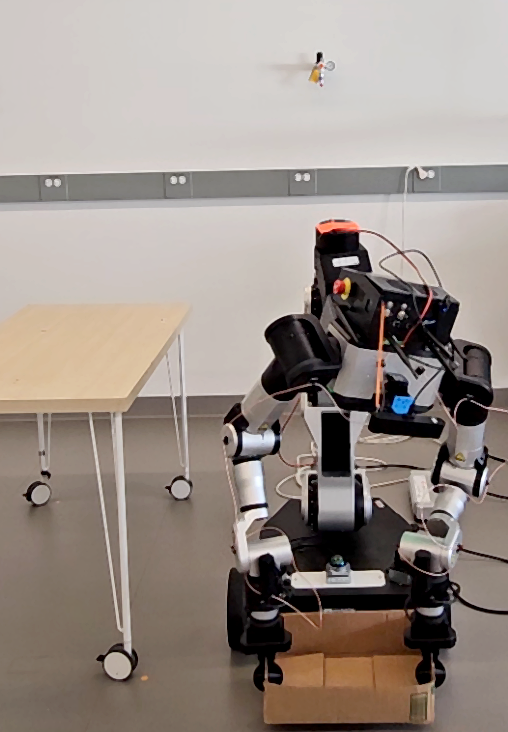
\includegraphics[width=0.45\linewidth]{images/ruby1.png}%
    \hfill
    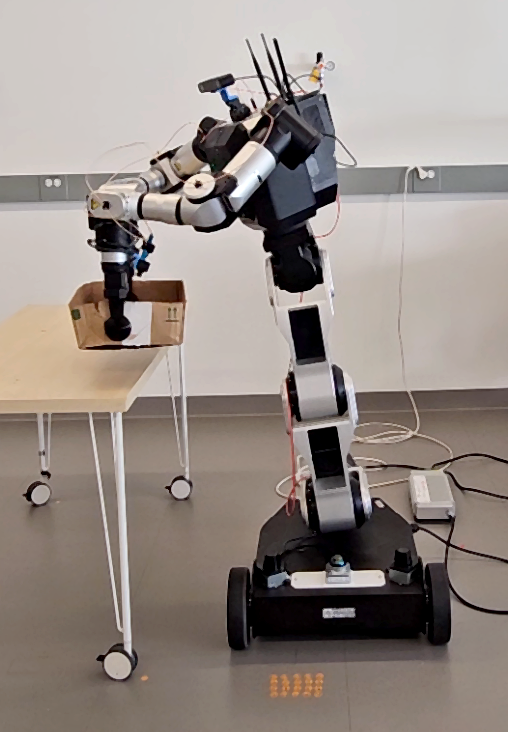
\includegraphics[width=0.45\linewidth]{images/ruby2.png}
    \caption{A 23-DoF bimanual mobile manipulator performing a whole-body pick-and-place task with motion plans generated by our motion planner.}
    \label{fig:ruby_box}
    \vspace{-1em}
\end{figure}
% McVAMP, however, satisfies constraints only up to $\epsilon$-tolerances, and the iterative procedure of projection introduces synchronization dependencies that reduce parallelism efficiency.
% Despite the performance, projection based methods suffer from 3 key drawbacks: (1) some constraints, such as the bimanual-constraint collapse the effective planning space (14-DoF to 8-DoF), making planning in the full ambient space highly inefficient. (2) Since projection is a sequential numerical procedure, so planning time is upper-bounded with high variance; constraints are satisfied only up to an $\epsilon$-tolerance at knot points, not continuously, so further projection along the curve is often needed. (3) Projections distort the underlying geometry (since they encourage projections on the boundary), so configuration-space distance and neighborhood no longer reflect task-space structure.
% \tccomment{Drawbacks (2) and (3) are pretty technical (especially 2), and I don't think you need to call out McVAMP as flawed in order to justify this work. Perhaps phrase it as ``McVAMP brought VAMP to one class of algorithms for CMP, we bring it to another class of algorithms''. Then you can talk about why we might like parameterization-based methods, and then follow it up with our (more-technical) observations about why parameterization algorithms are actually better-suited to VAMP-style parallelism.}
% . It exploits known mappings of a robot such as forward kinematics, and its differentials by pre-compiling the instructions for collision checking and constraint projection inside the planning operations, which unlocks magnitudes of speed-up in performance, while maintaining guarantees at the same time. These works have closed the real-time gap and have made real-world operation possible. 
% Despite the impressive performance, projection based manifold constraint methods suffer from certain drawbacks. (1) Some constraints, such as the bimanual-constraint, significantly lower the dimensionality of the planning space, from 14DoF to 8DoF, which makes planning in the 14DoF space highly inefficient. (2) Since they use numerical procedures to converge onto a manifold, planning times are upper-bounded by the sequential nature of projection, which could have large variances. Constraints are often satisfied only upto certain epsilon-tolerances and only at the knot points, instead of every single point in the trajectory, and computing constraint-satisfying trajectories could require further projection step along the curves, increasing system times. (3) These projections often distort the underlying geometry (since they encourage projections on the boundary), so notions of distance and neighborhood in configuration space may not accurately reflect those in the task space -- in practice it makes steering and nearest-neighbor operations non-trivial for planning and produces long-winded paths. Finally, these planners require constraint-satisfying joint configurations as initial conditions, which are not always easy to find.
% <TOMMY, motivate the need for sequential planning> 
% <introduce analytic parameterization of IK>
 % Analytic IK parameterization on the other hand provide a compact representation of the end-effector constraint space, using a deterministic mapping between end-effector constraint and joint configurations.~\cite{tommy} demonstrate the use of 
% - Whats CMP? — example of a bimanual lift, example of stability in planning etc —> all the good stuff
% - How they’re currently solved : mcvamp —  super fast etc
%     - But it is a numerical procedure and is iterative, which makes it inherently sequential — it is bounded by the iterations taken to converge onto a manifold. Due to this sequential nature, the variance in planning times could be large, especially for hard or impossible problems.
%     - Samples in a higher dimension and projects onto a lower one — which makes it inefficient as the d-m grows.
%     - often constraints are expressed in the end-effector space and not in configuration space —> one of the drawbacks of mcvamp is the need to have a valid IK for both the start and goal configurations to lie on the manifold which is a rough ask
%     - Since it is a numerical procedure, it can respect constraints only at knot points, and intermediate configs need further projection which is also time-consuming.

Although the constraint manifold reduces the feasible space dimensionality, vectorized planners still operate in the full-dimensional ambient space, and rely on fast projections to accelerate  planning. We instead bring this vectorization paradigm to another class of CMP methods based on reparameterizing the planning space. These methods define a lower-dimensional planning space from the constraints, satisfying them by construction, reducing the dimensionality of the planning problem. For instance, a 14-DoF space, subjected to a bimanual constraint can be reduced into a 8-DoF planning space, avoiding sampling and projection in the ambient space. Parameterization using analytic inverse kinematics have been used to plan in task-space and then map back to joint configurations~\cite{cohn2024constrained}. 
The analytic reparameterization effectively eliminates the corresponding equality constraint from the motion planning problem, turning it into an unconstrained problem. However, these planners are often bottlenecked by the need to call IK hundreds to thousands of times for validation, which dramatically increases the planning time due to the latency of invoking the IK routine.
% and the branching logic inherent to analytic IK makes each of these calls expensive. 
% \tccomment{I don't think the branching logic makes it slow?}

At the same time, this formulation lends itself more naturally to vectorized execution. Unlike iterative numerical projection whose computation time depends on the convergence, analytic IK evaluates a predetermined, non-iterative sequence of operations for each planning state. 
This is repeatable across planning states, making it well-suited to SIMD-style execution. 
% \tccomment{Need to define SIMD earlier, maybe when first introducing VAMP?}
% in whose underlying metric is more meaningful to the task-constraints, preserving notions of distances and neighborhoods.
% \tccomment{I'd be careful about saying that the analytic parameterization yields good geometry -- it actually doesn't a lot of the time. I'd focus on the fact that parameterization effectively eliminates the equality constraint, yielding an ``unconstrained'' problem.}
Crucially, similar to forward kinematics, the analytic IK mapping is also a fundamental property intrinsic to the kinematics of a robot, and thus can be precompiled once for a given robot. Its implementation can be specialized and optimized for the underlying hardware. 
% \tccomment{I think this is the place to talk more about why parameterized planners are better suited to VAMP-style parallelism than projection-based planners}
% \tccomment{Suggest combining all content after this comment into a single paragraph stating our contributions. ``We made this planner. It uses X methods to make it awesome. It solves Y problems at Z speed. It is so fast that it changes how we design real-world robotics pipelines, as we demonstrate on the RB-Y1 experiment.''}
% \sicomment{unfortunately the following did not work}
% In addition to speeding up planning, we explore two axes of parallelization — (i) planning on a single IK branch and (ii) generate constraint-satisfying inverse kinematics across all IK branches. 
% Since most real-world constraints show up as end-effector constraints, a natural coordinate system for planning is the end-effector $SE(3)$ space. Using analytic inverse kinematics (IK), one could go between end-effector space and the joint configuration space for robot control~\cite{cohn2024constrained}. 
% The analytic reparameterization defines a space in which the underlying metric is more meaningful to the task-constraints. Consequently, distances and neighborhoods in this space are more geometrically consistent. It enables a compact representation and allows directly sampling on the constraint space, which can improve the efficiency of planning. In addition, a generated trajectory in this space strictly adheres to the constraint upto any resolution, which is critical for sensitive systems. 
% SEW (shoulder-elbow-wrist) arms, they do blah blah, which can generate 16 different modes of solutions. 
% Due to these things, and thus are amenable to pre-compilation.
% Using the property of the robot, (upto 16 branches), and construct . These methods can be embarrassingly parallelized, since they typically contain a fixed set of instructions, unlike iterative projection based methods. 
% On the other hand, analytic parameterization of inverse kinematics can handle task-space constraints more naturally, since end-effectors lie in the same space as the constraints. Parameterizing enables a compact representation and allows directly sampling on the constraint space, which can improve the efficiency of planning. In addition, a generated trajectory in this space strictly adheres to the constraint upto any resolution, which is critical for sensitive systems.
% In addition to simply vectorizing planning operations, the Vector Accelerated Motion Planner decouples inherent properties of a robot from external ones. It exploits these known mappings of a robot such as the forward kinematics, by pre-compiling the instructions for collision checking inside the planning operations, which unlocks magnitudes of speed-up in performance, while maintaining guarantees at the same time. McVAMP similarly precompiles the differentials of the forward kinematics, which are then used for numerical projection to the constraint manifolds. This begs the question: what other properties that are inherent to a robot can be pre-compiled efficiently and exploited during planning?  

To this end, we explore a new axis of precompilation and subsequent vectorization for an accelerated planner that uses an analytic parameterization to plan in end-effector constrained spaces. Our proposed planner runs on a single core CPU and generates constraint-satisfying plans in real-time, ranging from microseconds for 7-DoF systems to milliseconds for a 20-DoF bimanual mobile manipulator. Planning in end-effector space further enables early collision detection and predictable per-iteration computation. We finally demonstrate how this increased throughput can enable new possibilities for sequential manipulation pipelines for a humanoid pick-and-place task. 
% In addition to the speed, planning in this space allows other benefits such as early collision detection, and the ability to "upper-bound" per-iteration planning times, thereby improving long-tail cases. 

% \sitotccomment{is this needed or we remove it altogether?} \tccomment{See above, think it's good to include, but condense a bit.}
% Finally, we revisit the problem of a sequential manipulation problem using the planner, where the robot has to synthesize a sequence of actions, all of which need to be chained together to be feasible. With the increased throughput of the planner, we essentially restructure the pipeline, we can evaluate many more potential actions, producing shorter overall trajectories at a faster rate.   


\section{Related Work}
Constraint motion planning is a well-studied problem due to its applicability to the real world. Several approaches have been proposed for CMP, which can broadly be classified into optimization-based, sampling-based, and learning-based methods. Optimization based methods~\cite{dragan2011manipulation, schulman2014motion,sundaralingam2023curobo1} typically treat the constraint as a soft-penalty term in their planning objective. But they can only satisfy the constraints weakly and can get stuck in local minima.
% \tccomment{Can condense the description of SBMP a lot. Suggest phrasing it as ``SBMPs must leverage specialized routines to draw samples from the measure-zero constraint manifold [cite Zak review], such as projection [citations] or numerical continuation [citations].''}
Sampling-based planning methods (SBMP) must leverage specialized routines to draw samples from the measure-zero constraint manifold~\cite{kingston2018sampling}, such as projection~\cite{berenson2009manipulation} or numerical continuation~\cite{jaillet2013atlasrrt, kim2016tangent}, which can all be abstracted away in standard SBMP methods~\cite{kingston2019exploring}.
% have shown to be extremely effective at producing constraint-satisfying plans in complex environments, by relying on various sampling on the constraint manifolds and constructing a graph structure. Projection-based SBMP methods~\cite{berenson2009manipulation} projects using iterative numerical methods, while continuation-based approaches~\cite{jaillet2013atlasrrt, kim2016tangent} maintain piecewise approximations of the manifold's tangent space for traversal. 
However, sampling from constraint manifolds is often an expensive operation, they may satisfy constraints only up to $\epsilon$-tolerances, which may not be sufficient for sensitive systems. The distorted paths are also not straightforward for a controller to execute. 
% \tccomment{phrasing}
% \tccomment{Suggest condensing. First sentence unchanged, but cite everything in that sentence. Drop second sentence. Focus third sentence on need for retraining and catastrophic learning error (discontinuities in the latent space, see ``A Constrained Motion Planning Method  Exploiting Learned Latent Space for High-Dimensional State and Constraint Spaces'').}
Learning based methods attempt to learn a constraint, so that sampling and traversing the manifold can be done directly in the latent space of a neural network~\cite{qureshi2020neural, qureshi2021constrained, ni2024physics}.
% CoMPNet~\cite{qureshi2020neural} and CoMPNetX~\cite{qureshi2021constrained} are trained using imitation learning from a dataset collected using sampling based planners, while C-NTFields~\cite{ni2024physics} uses a physics informed neural networks to compute an edge to lie on a manifold. 
But these methods require time-consuming retraining for new constraints, for which data collection may not be easy.

Yet another line of research attempts to directly sample the constraint manifold, using numerical or analytical IK to recover joint configurations~\cite{cortes2005sampling, han2001kinematics, wang2019inverse, lee2014prot}. Cohn et al.~\cite{cohn2024constrained} extend this idea by constructing parameterizations tailored to bimanual constraints and using the resulting IK mappings to reduce the dimensionality of the search space. Most of these methods leverage analytic IK routines to resolve parameterized configurations back into joint-space configurations for collision and validity checking. Tools such as IKFast~\cite{ikfast}, IK-Geo~\cite{elias2025ik} and SSIK~\cite{ssik} can be used to automatically generate analytic IK solutions for a wide range of arms. 
% \tccomment{Recommend not citing Paro, it's mathematically very dubious (check out \S III.B if you're interested). I made an overleaf comment with earlier IK parameterization papers.}
% Works such as KPIECE~\cite{csucan2009kinodynamic} have shown that compacting the search space (especially with a task-space bias) can dramatically speed up motion planning. 
% These methods can also be combined with optimization based procedures for satisfying other goals.~\cite{cohn2026framework}. 
Yet, these methods are often bottlenecked by the IK computation at each step of planning to perform validity checking, which slows down the planner. Our work is strongly inspired by this class of methods, and attempts to specifically address the computational cost of IK during planning.


% \textbf{Inverse Kinematics}
% \tccomment{Do we even need to review IK methods in related work at all? Suggest just adding the citations in the above paragraph, and mentioning specific facts with citations as needed later in the paper.}
% The problem of recoving joint configurations that satisfy desired end-effector poses is the well-studied problem of inverse kinematics (IK). Unlike the forward kinematics (FK), IK is a set-value mapping, i.e. multiple joint configurations satisfy a given pose. This ambiguity is particularly important for robot arms with greater than 6 degrees of freedom, where the set of solutions lie on different, possibly disconnected branches, called self-motion manifolds. Burdick~\cite{burdick1989inverse} showed that there at most 16 different branches for robot arms in 3D space, with each branch admitting infinite solutions.

% Existing approaches can generally be classified into (1) optimization-based and (2) analytic methods. Optimization IK constructs a non-linear optimization problem and iteratively search for a solution using methods such as gradient-based optimization or non-linear programming. However, numerical methods are often time-consuming and are not guaranteed to find a solution. 

% Analytic IK on the other hand derives closed form equations from the kinematic structure to tackle the problem, and most solutions attempt to enumerate solutions from all branches. For kinematically redundant robots, analytic solutions introduce one or more \emph{free parameters} to resolve the remaining redundancy. These parameters can be resolved either by locking selected joints or by specifying a desired value for the free parameter and recovering the corresponding joint configuration. A substantial body of work has focused on deriving and automating IK solutions. Various hand-crafted solutions have been developed for individual robots, such as the ones for Franka Emika Panda~\cite{franka_ik2021}, KUKA Iiwa, and the UR5. Due to the manual effort needed to designing these IK, several approaches have been proposed to automate this generation, exploiting algebraic structures in kinematics. Perhaps the most widely used tool is IKFast~\cite{ikfast}, which performs symbolic manipulation to derive closed form equations for joint angles to then do code generation. More recent works attempt to expand the range, reliability and readability of IKFast. EAIK~\cite{eaik} performs subproblem decomposition to identify known kinematic structures, and composes their solutions. IK-Geo~\cite{} propose a semi-analytic IK for solving 6R robots, employing 1D line search methods for final resolution. Finally, ~\cite{ssik} combines most of these methods to provide a reliable certifiable solution. 

% Most solutions attempt to exploit the kinematic structure of the arm, in order to automate the generation of IK. Need to mention ikfast, geofik, ssik, 16 branches, smm etc. 

% The analytic inverse kinematics mapping is an inherent property of the robot's kinematic structure. Tools such as IKFast~\cite{ikfast} can derive closed-form IK solutions for a broad class of manipulators, which often produce multiple discrete solution modes. For example, SEW arms (shoulder-elbow-wrist) admit up to 16 discrete branches~\cite{16branches}. These methods can be embarrassingly parallelized, since they contain a fixed set of instructions, unlike iterative projection based methods. 


% <also talk about kpiece that shows planning in lower dimensional space>

% \textbf{Talk about accelerating planners}

%\textbf{Accelerating Motion Planning through Parallelism:} 
To improve the throughput of motion planning, works have focused extensively on using parallelism~\cite{amato1999probabilistic}, targeting different pieces of the pipeline. Some methods perform multiple SBMP iterations in parallel, while others run multiple searches in parallel~\cite{cforest}. cuRobo~\cite{sundaralingam2023curobo1} uses GPU parallelism to perform multi-seed optimization-based motion planning, treating constraints and collisions as penalty terms to the objective. VAMP~\cite{vamp} on the other hand takes a fine-grained approach and uses CPU SIMD operations to parallelize collision-checks for edge validation within a planning iteration, which has shown orders of magnitude performance boost. McVAMP~\cite{iyer2026vectorizing} similarly parallelizes the projection operations inside a planning iteration onto a manifold for constraint motion planning, which also demonstrates an equivalent speedup. However, it is still bottlenecked by the iterative projection procedure, which could arbitrarily stall the pipeline. Empirically, for a 7-DoF arm with a plane constraint, it spends 16\% of its projection time waiting for the last sample to converge.
% \tccomment{If we have numerical results that show how much ``waiting'' the parallel projections causes, we could name drop that here specifically. Or we could just say ``...iterative projection procedure, which is fundamentally challenging to parallelize''.}
We follow a similar approach, and attempt to use fine-grained parallelism to resolve the IK bottleneck, by performing analytic IK in parallel, which is more suited to vectorization.
% VAMP, Curobo, learning-paper, McVAMP


% \textbf{Sequential multi-modal planning:} Often sequential manipulation often seek to reduce the number of expensive motion planning queries, by imposing additional structures on the problem. Such approaches leverage prior experience~\cite{kingston2021using}, similarity~\cite{hu2024motion}, exploration/exploitation tradeoffs~\cite{garrett2020pddlstream}, downsampling~\cite{jiao2025integration} or deferring motion planning until after cheap pre-filtering and grounding~\cite{khodeir2023policy, wang2022lazy}. Despite the success of these methods, they have significant overheads, owing to the structures required to guide the search. In contrast, with advances in improving the efficiency of motion planning computations, recent works like SPaSM~\cite{spasm} instead increase the amount of sampling and motion planning computations by exploiting the parallelism offered by GPUs. 

% also need to talk about multimodal sequential planning.
% To talk about:
% Whole-body motion planning has been extensively studied for high-dimensional robots, particularly humanoids and mobile manipulators. 

% let us make it nicer, and start motivating from an aspect of whole body solving problem

% \begin{enumerate}
%     \item Motion planning and then VAMP
%     \item Constrained motion planning, and cbirrt, mcvamp and friends
%     \item The two parameterization papers - bimanual IK, combining sampling and optim IK
%     \item whole body planning
% \end{enumerate}



% In addition, the inverse kinematics is an inherent "property" of a robot. Tools like IKFast can derive closed form inverse kinematics solution for a robot. VAMP exploits known mappings of a robot such as the forward kinematics, by pre-compiling the instructions for collision checking inside the planning operations, which unlocks maginitudes of speed-up in performance, while maintaining guarantees at the same time. This begs the question: what other properties that are inherent to a robot can be pre-compiled efficiently and exploited during planning, and the ik mapping serves as a natural candidate for it. In addition, due to its closed-form nature, IK can be can be embarrassingly parallelized.

% \callout{Need to talk about GCP branches somehow}


% To that end, we propose a parameter-space vector accelerated planner that can generate constraint-satisfying plans in under a millisecond for most problems. Through this formulation, we explore two axes of parallelization — (i) and (ii) generate constraint-satisfying inverse kinematics across all IK branches.



% Another benefit of the parameterization over iterative sequential procedures is the ability to "upper-bound" the time taken at each step of planning, thereby reducing the total variance for impossible problems.

\section{Preliminaries}
\label{sec:prelim}

Let $C \subset \mathbb{R}^d$ be the configuration space of a robot with $d$ degrees of freedom, where a configuration $q \in C$ is typically the vector of actuated joint angles.
In the presence of environment obstacles, $C_\text{free} \subset C$ denotes the subset of configurations that are not in collision.
%\begin{definition}[Motion Planning]\label{def:mp}
%Given $q_\text{init}, q_\text{goal} \in C_\text{free}$, find a continuous path $\sigma : [0,1] \to C$ such that
%\begin{equation*}
%  \sigma(0) = q_\text{init}, \quad
%  \sigma(1) = q_\text{goal}, \quad
%  \sigma(t) \in C_\text{free} \; \forall t \in [0,1].
%\end{equation*}
%\end{definition}
A robot typically interacts with the environment through its end-effector(s), EE(s).
The forward kinematics map $\FK : C \to SE(3)$ gives the EE pose of a configuration and defines the task space reachable by the end-effector,
\begin{equation*}
  T = \FK(C) = \{\, \FK(q) \mid q \in C \,\} \subset SE(3).
\end{equation*}

In constrained motion planning (CMP), the path must additionally satisfy task constraints, typically expressed on $C$ by an implicit constraint function $F : C \to \mathbb{R}^k$, where $k$ is the dimensionality of the constraint.
This defines a lower-dimensional constraint manifold and its collision-free subset,
\begin{equation*}
  M = \{\, q \in C \mid F(q) = 0 \,\} \subset C, \quad
  M_\text{free} = M \cap C_\text{free}.
\end{equation*}

\begin{definition}[Constrained Motion Planning]\label{def:cmp}
Given $q_\text{init}, q_\text{goal} \in M_\text{free}$, find a continuous path $\sigma : [0,1] \to C$ such that
\begin{equation*}
  \sigma(0) = q_\text{init}, \quad
  \sigma(1) = q_\text{goal}, \quad
  \sigma(t) \in M_\text{free}, \forall t \in [0,1].
\end{equation*}
\end{definition}

Since $M$ has measure-zero in $C$, instead of uniform sampling, sampling-based CMP must generate samples on $M$ by other means~\cite{kingston2018sampling}.
Projection-based CMP~\cite{berenson2009manipulation} maps a sample $q \in C$ onto $M$ with an iterative operator $\Proj_M(q)$ that drives $F(q)$ to zero using Newton updates on $\partial F / \partial q$.

A widely used class of constraints restricts the EE pose to a subset $T_c \subset T$, itself defined implicitly by a function $g : SE(3) \to \mathbb{R}^k$,
\begin{equation*}
  T_c = \{\, X \in SE(3) \mid g(X) = 0 \,\}.
\end{equation*}
This induces the configuration-space constraint $F(q) := g(\FK(q))$, so that $M = \{\, q \in C \mid \FK(q) \in T_c \,\}$. This encompasses constraints ranging from keeping a glass level to fixing both feet of a humanoid to the ground.
% This encompasses both simple constraints like holding a glass of water level and complex constraints like keeping both feet of a humanoid fixed on the ground.

Inverse kinematics is the preimage of a pose under $\FK$,
\begin{equation*}
  \IK : SE(3) \rightrightarrows C, \qquad
  \IK(X) = \{\, q \in C \mid \FK(q) = X \,\}.
\end{equation*}
Unlike $\FK$, $\IK$ is set-valued, as a single pose admits multiple solutions. Specifying a discrete branch $b$ and a continuous self-motion parameter $\psi \in \Psi$ gives a single-valued map $q = \IK_b(X,\psi)$
where $b$ selects a self-motion manifold (SMM) and $\psi$ parameterizes it~\cite{burdick1989inverse}.
% To write $\IK$ as a function, one must specify a discrete branch $b$ selecting a self-motion manifold (SMM) (e.g., elbow-up vs.\ elbow-down) and, for redundant arms, a continuous self-motion parameter $\psi \in \Psi$ (e.g., a redundant joint angle for a 7-DoF arm)~\cite{burdick1989inverse}.
% A pose, branch, and self-motion parameter then uniquely determine a configuration $q = \IK_b(X, \psi)$.
This leads to an interpretation of $\IK$ as a nonlinear change of coordinates on $C$. 
% \tccomment{phrasing}
Many EE constraints admit simple descriptions of $T_c$ (e.g., bimanual carrying is an affine constraint between the two EEs), so this change of coordinates yields a chart $M$.

When the end-effector constraint can be expressed functionally, the planning problem can be reparameterized~\cite{cohn2024constrained} to operate in a parameter space $\mathbb{P}$ instead of $C$.

\begin{definition}[Reparameterization]\label{def:reparam}
A reparameterization of $M$ is a pair $(\mathbb{P}, \Phi)$ of a parameter space $\mathbb{P}$ and a map $\Phi : \mathbb{P} \to C$, continuous where defined, such that $\Phi(\mathbb{P}) \subseteq M$.
\end{definition}

Every parameter thus satisfies the constraint by construction.
In our case, $\Phi$ is built from analytic $\IK$, e.g., for a redundant arm constrained to a plane with fixed orientation, $\mathbb{P} = \mathbb{R}^2 \times \Psi$ and $\Phi(p) = \IK_b(X(p), \psi)$, where $X(p) \in T_c$ is the pose determined by $p$.
Where $\IK_b$ has no solution (unreachable pose or joint limits), $\Phi$ is undefined and $p$ is invalid---we treat this similar to collision.
Conversely, a configuration $q \in M$ is mapped to $\mathbb{P}$ by $\Phi^{-1}(q)$, computed from $\FK(q)$ together with the branch and self-motion parameters recovered from $q$; this is how $q_\text{init}, q_\text{goal}$ are lifted to $p_\text{init}, p_\text{goal}$.
Sampling and interpolation in $\mathbb{P}$ are closed-form, and, unlike $M_\text{free} \subset C$, the collision-free parameter set
\begin{equation}\label{eqn:pfree}
  P_\text{free} = \{\, p \in \mathbb{P} \mid \Phi(p) \in M_\text{free} \,\}
\end{equation}
has positive measure in $\mathbb{P}$, so uniform sampling in $\mathbb{P}$ yields constraint-satisfying samples directly.

\begin{definition}[Reparameterized Motion Planning]\label{def:rmp}
Given a reparameterization $(\mathbb{P}, \Phi)$ and $p_\text{init}, p_\text{goal} \in P_\text{free}$ with $\Phi(p_\text{init}) = q_\text{init}$ and $\Phi(p_\text{goal}) = q_\text{goal}$, find a continuous path $\tau : [0,1] \to \mathbb{P}$ such that
\begin{equation*}
  \tau(0) = p_\text{init}, \quad
  \tau(1) = p_\text{goal}, \quad
  \tau(t) \in P_\text{free} \; \forall t \in [0,1].
\end{equation*}
\end{definition}

A solution $\tau$ to \cref{def:rmp} yields a solution $\sigma := \Phi \circ \tau$ to \cref{def:cmp}, since $\sigma$ is a composition of continuous maps.
The converse holds only within a single chart: a CMP solution $\sigma$ lifts to a path in $\mathbb{P}$ when $\Phi$ is a homeomorphism onto its image along $\sigma$, i.e., when $\sigma$ stays on one SMM branch $b$ away from kinematic singularities.
Solutions that cross branches are not captured by a single $(\mathbb{P}, \Phi)$; the parameterizations used for each robot are discussed in \cref{sec:expts}.

A noteworthy benefit of planning in the reparameterized space is that often, start-goal planning queries are easier to specify in the EE/parameterized space, rather than joint configurations on the constrained manifold space.

\section{Methodology}
% \tccomment{Still making comments in this section, but deferring to Shru/Zak since I haven't written this sort of thing before}
In this work, we propose a new compilation axis for a robot: the analytic inverse kinematics routine, and the subsequent reparameterization that is constructed from it. Starting from the analytic solver, we transform the generated routines into branchless and vectorizable units that map parameterized configurations into joint configurations in parallel. This allows multiple configurations in the reparameterized space to be resolved simultaneously using SIMD parallelism. Finally, we integrate it into the sampling based planner, to accelerate the edge-validation of the planner.
% Since edge-validation requires every configuration along the edge to satisfy the constraint and be collision-free, while exploiting the all-or-nothing nature of edge validity.

\subsection{Analytic IK Compilation to generate the parameterization}
\label{sec:compileik}
The primary goal of reparameterization is to define a new planning space $\mathbb{P}$, along with mappings between it and the robot's joint configuration that enable planning operations. We generate this mapping using standard analytic IK tools such as IKFast~\cite{ikfast}. However, IKFast generates instructions with conditional statements that prevent trivial parallelization. Fortunately, these conditionals follow a specific structure that can be eliminated; consequently, we carefully modify in two stages to produce a branchless instruction set that is vectorizable. 
% Let the total number of SMM branches be denoted by $k$. According to ~\cite{16}, there are atmost 16 different SMM branches for an arm in $SE(3)$ space. 
\begin{enumerate}
    \item At the highest level, it is split into $k$ templated initializations, one for each SMM branch defined by the sign for shoulder, wrist and elbow, so that no branch selection happens at runtime. According to ~\cite{burdick1989inverse}, there are at most 16 distinct branches where solutions lie for arms operating in $SE(3)$.
    % \tccomment{I would name drop the Burdick up-to-16-solutions fact here.}
    \item For a fixed SMM branch, data-dependent logic such as guards for inverse trigonometric operations, angle-wraps, and wrist kinematic singularities are replaced with safe branchless versions, by relaxing them into a saturation loss instead of hard clamps. An IK solution is valid if the losses are all negative, and if the returned configuration lies within joint limits. This is analogous to the reachability probing functions in \cite[\S 4]{cohn2026framework}.
\end{enumerate}

These inverse kinematics are then used to generate the parameterized space, depending on the constraint-class. For a 7-DoF arm, it consists of the end-effector $SE(3)$ pose along with $\psi$. For a bimanual 14-DoF with a fixed relative transform constraint between the end-effectors, a single arm $SE(3)$ pose suffices. These parameterized spaces for each robot and constraint are discussed in~\cref{sec:expts}. 

The next step is to compile these parameterizations for planning. Similar to VAMP, we expand the tracing compiler built on top of Pinocchio~\cite{carpentier-sii19} and CppAD~\cite{cppad} to generate a branchless loop-free compiled instruction set for the IK and its subsequent parameterization.
% Since the analytic IK is smooth with respect to $\psi$ within a branch, we also use the same compiler to generate the instruction set for its differential with respect to the free-parameter. 
Within the analytic IK function, inverse trigonometric operations are approximated using polynomials \tccomment{would we cite something here? I would appreciate as a reader}\sicomment{its from cephes which is ancient and industry standard}, and a smooth hinge loss is applied for reachability probes. We additionally compile the distance and interpolation operations on this new space. For pose components, we use spherical linear interpolation and a smooth $SO(3)$ geodesic, with their Euclidian counterparts for translation. For parameterizations that combine joints with IK~\cref{expts:ruby}, the interpolations and distance are split into linear interpolation and Euclidian distance for the joints, and $SE(3)$ operations for the pose.

A noteworthy benefit of compiling the IK function is its modularity: we can parameterize many constraint manifolds in terms of a single IK implementation, and therefore plan paths on them without recompliation.
% \tccomment{If there are specific functions within analytic IK that require specialized treatment (or at least, weren't considered in prior work), I think it's worth citing them. Trig functions are the main one that come to mind -- I didn't know how that was done until you told me. Inverse trig in particular, I would have thought it's a problem near the edges, and it's not -- worth explaining why.}


% <make sure to introduce the term resolution of the parameterization>

% \tccomment{Suggest moving most of the following paragraph to subsection C, where you talk about the other motion planning stuff. Can just conclude here with noting that analytic IK is the primitive you need for parameterized-planning, and now you've made it fast and vectorizable. And maybe name drop the portability/modularity.}

\subsection{Vectorizing the trace compiled operations}

With this approach, the compiled instruction set now takes a parameterized space input $p \in \mathbb{P}$ and directly generates a joint configuration $q \in C$, along with validity, given by $\Phi : \mathbb{P} \to C$. In the sampling based planner, the sampled ``configurations", tree/graph structure, and motion validation, all exist within this new parameterized space. Since the space is constructed out of the task-enforced constraint by structure, all valid states in it naturally satisfy the constraint without extra operations. However, satisfying the constraint alone is not enough: conventional collision and joint-limit checking are still needed to ensure configuration validity.
% \tccomment{Need to describe the additional constraints we have to satisfy here (reachability and follower arm joint limits). Suggest pointing out the following facts: (1) still the ordinary rejection-sampling framework used for collisions, and (2) simpler to compute than collision checking -- joint limits requires no FK, reachability probably doesn't (depends how you use the saturation values).}



% \paragraph{Resolution of multiple goal-poses}
% <talk about reparameterized space, admits complex mappingsm distance nicer>p
Similar to VAMP, we vectorize the computation of IK using SIMD for its minimal overhead. Eliminating conditional logic enables us to repack the instruction set's input from an array-of-structures (AoS) into structure-of-arrays (SoA). The same IK routine can then process multiple parameterized space inputs simultaneously to obtain their corresponding joint configurations. The degree of parallelism is determined by the specific architecture the planner runs on; AVX for instance holds eight 32-bit floating points per register, letting us resolve 8 inputs in parallel.


% \subsubsection{Vectorizing across the IK branches}
% \paragraph{Resolution of a single goal-pose across multiple IK branches}
% We also propose a similar, yet subtly different axis of vectorization: resolving the same parameterization across multiple IK-branches in parallel. 7-DoF arms admit only upto 16 distinct self-motion manifold branches, and most 7Dof systems in practice resolve only upto 8. This low cardinality is ideal for CPU based parallelization. Since the generated IK mappings are branchess and templated such that every branch executes the same instruction set, we vectorize the IK evaluation of a single goal configuration across these branches instead, where each SIMD lane computes the IK for a distinct branch.

\subsection{Accelerated Motion Planning using the parameterization}
% \begin{figure}
%     \centering
%     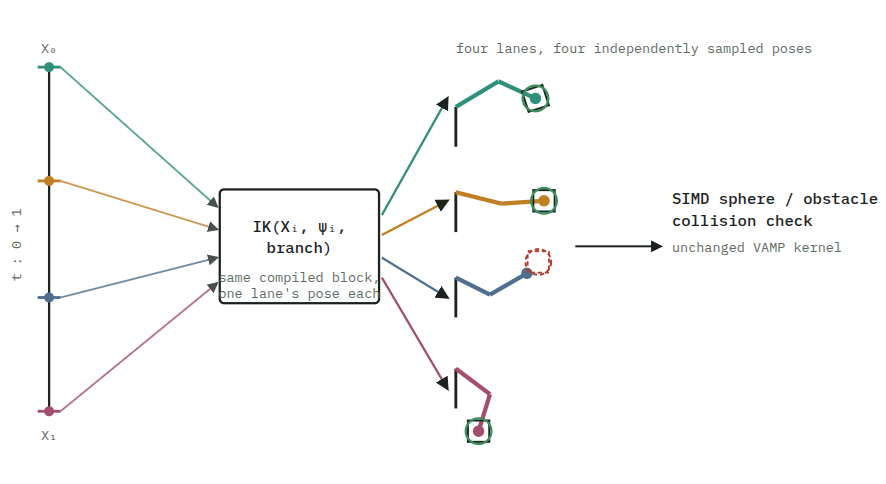
\includegraphics[width=0.99\linewidth]{images/methodology/pvamp_pic.png}
%     \caption{Four poses picked along a straight task-space interpolation feed the same compiled IK block, one pose per lane. Three arms close around their target; lane 3's gripper stops just short of its target and the marker is left hollow — a small, natural margin rather than a dramatic miss, since the sampled poses are themselves close together along the interpolation. \textbf{Dont come @ me zak for the AI fig pls. This is just a placeholder image of the general idea i want to convey}}
%     \label{fig:pvamp_local_planner}
%     \vspace{-1em}
% \end{figure}

% \begin{figure}
%     \centering
%     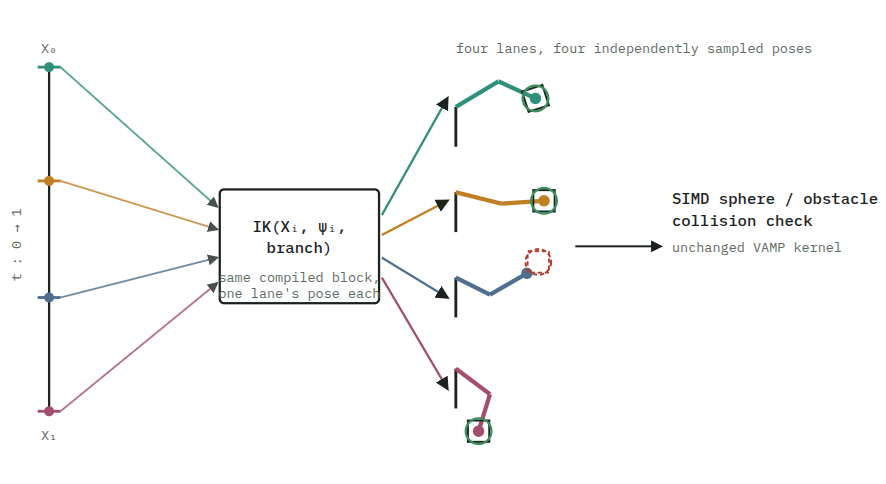
\includegraphics[width=0.99\linewidth]{images/methodology/pvamp_pic.png}
%     \caption{Space for a large image}
%     \label{fig:pvamp_local_planner2}
%     \vspace{-1em}
% \end{figure}
\begin{figure} 
% \centering
    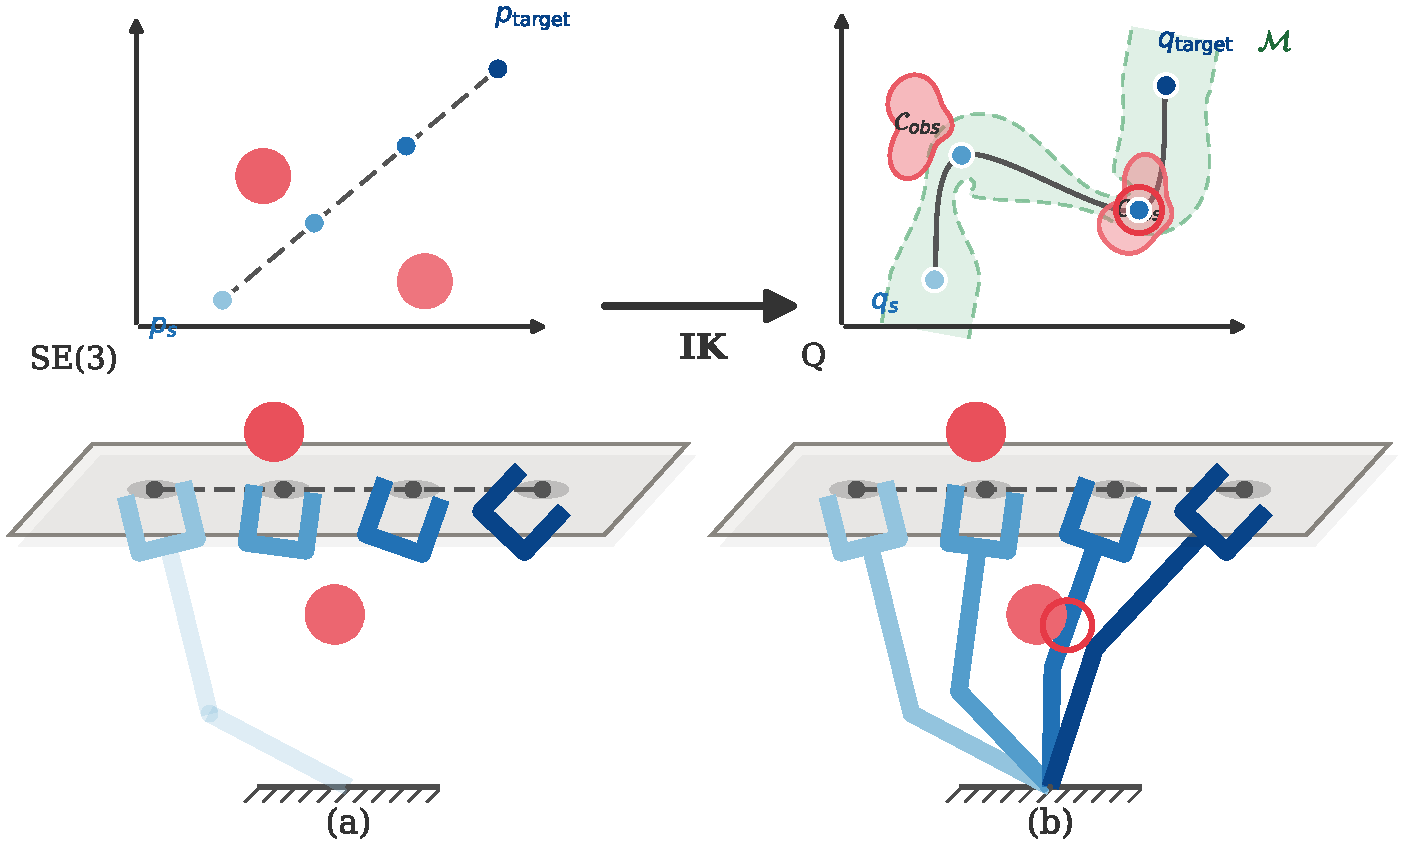
\includegraphics[width=1.0\linewidth]{images/methodology/robot_arm_fig_composite_start_eefs_all.pdf}
    \vspace{-1em}
    \caption{Vectorized Edge-validation in ReVAMP. Given $p_s$ and $p_\text{target}$ in parameterized space, they are interpolated, that are then validated in parallel. There are two stages here (a) Early-collision checking pre-filter by eliminating edges where the interpolated P-space points are in collision with the environment. (b) If EEFs are collision free, then IK is resolved in parallel and a full C-space collision check is performed. \textit{$n=4$ (unit of parallelization) here for illustrative purposes}}
\label{fig:methodology}
\end{figure}

% \sicomment{TODO add this While the parameterized space satisfies the equality constraint, standard collision checking is still performed at discrete points.}
 \begin{algorithm}[!htbp]
\caption{\contrib{ParameterizedExtend}}
\vspace{0.2em}
\label{alg:paramextend}
\footnotesize
\begin{algorithmic}[1]
\Require $\mathcal{T}, p_s, p_{\text{target}}, \Phi, \mathcal{E}, r, \rho$
\Procedure{ParameterizedExtend}{}
\State $\text{dist} \gets \Call{Distance}{p_s, p_{\text{target}}}$
\State $\text{reach} \gets \text{dist} < r$
\If{reach}
    \State $p_{\text{next}} \gets p_{\text{target}}$
\Else
    \State \contrib{$p_{\text{next}} \gets \Call{Interpolate}{p_s, p_{\text{target}}, r / \text{dist}}$} \Comment{\contrib{steer in $\mathbb{P}$}} \alglabel{algline:pe:steer}
\EndIf
\If{$\neg \Call{Accept}{p_{\text{next}}}$}
    \State \Return \textsc{Rejected}
\EndIf
\For{$i = 1$ \textbf{to} $\lceil \text{dist} / (n \rho) \rceil$} \Comment{$n$-wide SIMD blocks} \alglabel{algline:pe:loop}
    \State $p^{(1:n)} \gets \Call{InterpolateBlock}{p_s, p_{\text{next}}, i}$ \alglabel{algline:pe:interpolateblock}
    \If{\contrib{$\neg \Call{EefCollisionFree}{p^{(1:n)}, \mathcal{E}}$}} \alglabel{algline:pe:eefprefilter}
        \State \contrib{\Return \textsc{Trapped}} \Comment{\contrib{IK-free collision prefilter}}
    \EndIf
    \State \contrib{$(\text{valid}, q^{(1:n)}) \gets \Phi\big(p^{(1:n)}\big)$} \Comment{\contrib{batched IK}} \alglabel{algline:pe:ik}
    \If{$\neg \text{valid} \lor \neg \Call{CC}{\mathcal{E}, q^{(1:n)}}$} \alglabel{algline:pe:fkcc}
        \State \Return \textsc{Trapped}
    \EndIf
    \If{\contrib{$\neg \Call{JointContinuous}{q^{(1:n)}, \delta_{\max}}$}} \alglabel{algline:pe:jointdelta}
        \State \Return \textsc{Trapped} \Comment{\contrib{interlane $\ell_\infty$ jump check}}
    \EndIf
\EndFor
\State $\Call{AddVertex}{\mathcal{T}, p_{\text{next}}}$
\State $\Call{AddEdge}{\mathcal{T}, p_s, p_{\text{next}}}$
\If{reach}
    \State \Return \textsc{Reached}
\Else
    \State \Return \textsc{Advanced}
\EndIf
\EndProcedure
\end{algorithmic}
\end{algorithm}

An SBMP typically spends a significant amount of its time validating edges connecting two states, to which we bring the vectorization for acceleration, as detailed in~\cref{alg:paramextend}
% \tccomment{Haven't thought about it until now, but is this true for McVAMP? Or is more of the time spent on the projection (i.e. sampling)? I guess if you could projecting along an edge as part of the validation, it could still be the case. But maybe worth discussing?}\sicomment{In McVAMP, we took a slight detour, where sampling is done in free space, but projection happens only "during" edge validation, which was empirically much faster}\tccomment{I just want to be a little careful about the wording here. (I mean, asymptotically, nearest neighbors becomes the most expensive part of SBMP.) But maybe this is a trivial worry -- I'll defer to you and Zak.}
In the context of the parameterized planner, this requires sampling discrete points along the two states $p_s$ to $p_\text{target}$ up to a desired resolution~(\cref{algline:pe:interpolateblock}), transforming them back into configuration $q$ space to verify that (1) $q$ is valid and (2) $q$ is collision-free. First, we interpolate in the $\mathbb{P}$-space using closed-form interpolation operations that the parameterization provides between the start node $p_s$ and the target $p_\text{target}$~(\cref{algline:pe:interpolateblock}). For a motion/edge to be valid, every point along the edge needs to be valid.

% We exploit this requirement by early-exiting if any of the points tested in parallel fail to satisfy either one of the two conditions. 

To achieve this, we first use the vectorized IK and resolve operations across the different interpolated points to compute the joint configurations $q$~(\cref{algline:pe:ik}). Joint limits and reachability (using the saturation losses) can be checked in parallel from the IK without requiring forward kinematics. Then we use VAMP's vectorized broad-then-narrow-phase collision checking~(\cref{algline:pe:fkcc}) in parallel for the second condition. Since edge-validation has an all-or-nothing requirement, if any of the above checks fail even for a single point, the entire edge can be invalidated and exited early.

% , while collision checking is performed using VAMP's vectorized broad-then-narrow-phase procedure.



\textbf{Other tricks for efficiency:}
The end-effector is often the most-collision-prone link since it sweeps the largest space. Consequently, we first check the end-effector for collision at the sampled pose before IK~(\cref{algline:pe:eefprefilter}).
% This is made possible since our parameterized space is constructed out of the end-effector pose. 
This prefilter is possible because our parameterized space directly carries the end-effector pose, unlike joint-space samples, which requires forward-kinematics. This eliminates a significant number of IK calls and further denser collision checking in cluttered environments. Finally, to ensure joint-continuity for smoothness, we reject an edge if any two consecutively resolved configurations differ by more than 0.15 rad in any joint~(\cref{algline:pe:jointdelta}). Besides helping to avoid singularities, this improves reliability as the planner is forced to admit edges only to a bounded distortion subset of the manifold.
% \tccomment{Worth more discussion -- besides helping to avoid singularities and joint-space wraparound, this makes collision checking more reliable as it effectively forces you to plan within a bounded distortion subset of the manifold.}


% The extend extend step of our reparameterized planner is described in~\cref{alg:paramextend}.
% basically describe the vamp steps -- but add in this step. Also talk about early rejection Talk about being bottlenecked by needing to maintain joint continuity

% <both algorithms>
% <write algo>

% \subsection{Parameterization Space for different robots}
% \label{sec:arms}
% \sicomment{Make the notations consistent}
% \tccomment{Up to you if you want TSR, monogram, or something else. Suggest going with what you're most comfortable with.}

% Depending on the robot and the constraints enforced on its configuration by the task, the compiled IK is subsequently used to define the parameterized space $P$ explored by the planner. 


% \tccomment{A structural comment: since each experiment has its own parameterization, it might make sense to put the parameterizations in the experiments section? Could go either way, but I'm thinking it might be easier if readers see the parameterization in the context of the experiment it's used for.}

% \subsubsection{7-Dof FR3}
% The 7Dof Iiwa robot arm is the most straightforward case, where 
% For the 7-DoF Franka FR3 arm, we use the IK implementation provided by~\cite{franka_ik2021}. It produces solutions in 4 different IK branches, with one of the joint angles fixed as the redundancy parameter $\psi$. The 7-DoF arm is the most straightforward realization of the space. It takes in $X \in SE(3)$ pose and $\psi \in [-\pi, \pi]$ and the desired branch, and returns the configuration $q$. The parameterized space is now $X \times \psi$, which is 7-dimensional. This is ideal for tasks constrained by the end-effector, such as tracing a line/plane, and $X$ effectively becomes the new constrained space. (for eg. if the orientation is locked, it can just be $\mathbb{R}^3$). 
% \sitotccomment{need some help making it clear that we dont need to recompile for each new space, but we just restrict X during planning}
% \tccomment{See above: suggest putting it at the beginning of the section, since it's not just applicable to the 7-Dof FR3.}

% For the maze problem specifically, the end-effector is constrained to stay in a plane at a height $z = 0.22\,\mathrm{m}$ with locked roll and pitch; so in practice, parameterized planning collapses to $SE(2)$, with $X \in SE(2)$ with fixed values for the other dimensions, making it \textbf{4-dimensional}.


% \subsubsection{14-DoF Bimanual Iiwa Arm}

% \tccomment{In the context of a parameterized space requiring closed form sampling and interpolation, you should probably state how you do this for SE(3). (SLERP? Quaternions? Euler?)}

% \subsubsection{23-DoF Humanoid with a fixed base}
% \label{sec:rubyarms}

% In this setup, we use a Rainbow Robotics RB-Y1 mobile manipulator, which has two 7-DoF arms attached to a torso, which in turn is connected to the base by a 6-DoF chain, and a wheeled base. For the scope of this experiment, we disable the wheels, and fix the base to be at origin since we evaluate a pure manipulation task. Again, the goal is a bimanual-constrained box-transport task, whose constraints are similar to the 14-DoF Iiwa arm. In addition, it also needs to satisfy a stability constraint, where the center-of-mass (CoM) needs to lie within the support polygon of the base.

% % For the purposes of this setup, we fix the base to be at (0, 0, 0) and allow the other joints to move. 

% We use IKFast~\cite{ikfast} to generate the IK solution for the left and the right arms separately, and modify the generated IK solutions to be branchless as described in~\cref{sec:compileik}.
% It produces 8 different IK solution branches, with $\psi \in [0, 2\pi]$.
% \tccomment{Using ``branchless code'' in one sentence and talking about ``IK solution branches'' immediately after is confusing. Unfortunate overlapping terminology, but maybe ``The RB-Y1 arms have 8 disconnected self-motion manifolds, with redundancy parameterized by the angle of the $n$th joint (don't remember which).''}
% Similar to the bimanual iiwa, we implement a Task-Space IK setup. Given the torso joints, a mid-pose and a desired transform between the two arms, $T \in SE(3)$, the compiled instruction set first computes the goal pose of each arm, which is then passed through the respective per-arm IK mappings to obtain the desired configuration, while retaining the base and torso joints. Thus, the 23-DoF system is now parameterized to a \textbf{13-DoF space}, described as
% \[
%     \Phi : (q_\text{torso}, {}^{W}X^{B}, \psi_l, \psi_r) \mapsto (q_\text{torso}, q_l, q_r),
% \]
% where $B$ is the box frame and $\psi_{left}$ and $\psi_{right}$ are the arms' respective self-motion parameters.



% Honestly this section is pretty bare. Basically things to cover:
% - use IKFast/alternatives to generate ik for a robot, $psi$ parameter
% - implementation in the algorithm
% - early cc in this task space

% Bimanual planning. Two forms of parameterization

% Demonstrate planning there
% 1. Leader-follower setup
% 2. TaskSpaceIK setup


% Another axis of parallelization
% * parallelize over all 8 ik-branches, purely just sampling based, and show that ooo wee it works


% \begin{algorithm}[b]
\begin{footnotesize}
\caption{Reparameterized RRT-Connect}
\label{alg:crrtc}
\begin{algorithmic}[1]
% \zak{Why is the font so tiny??}
\Require $q_{a}, q_{b}, \mathcal{F}$

\State $T_{\text{a}} \gets \text{Tree}(q_{a})$, $T_{\text{b}} \gets \text{Tree}(q_{b})$

\While{$\text{iter} < \text{MaxIterations}$}
    \State $p_{\text{rand}} \gets \text{RandomConfigFromConstraint}()$ \label{algline:crrtc:rand}
    \State $q^a_{\text{near}} \gets \text{Nearest}(T_{\text{a}}, q_{\text{rand}})$ \label{algline:crrtc:near}
    \State $q^a_{\text{proj}} \gets \contrib{\text{ParallelConstrainedExtend}}
    (T_{\text{a}},
    q^a_{\text{near}}, q_{\text{rand}})$ \label{algline:crrtc:extend}
    \While{$q^a_{\text{proj}} \neq \textsc{NULL}$}
        \State $q^b_{\text{near}} \gets \text{Nearest}(T_{\text{b}}, q^a_{\text{proj}})$
        \State $q^a_{\text{proj}} \gets \contrib{\text{ParallelConstrainedExtend}}(
        T_{\text{a}},
        q^a_{\text{proj}}, q^b_{\text{near}})$
        \If{ $q^a_{\text{proj}} =q^b_{\text{near}} $}
            \State $\text{P} \gets \text{ExtractPath}(T_{\text{a}},  
            T_{\text{b}})
            $
            \State \Return \textsc{P}
        \EndIf
    \EndWhile
    % \zak{balanced? also dynamic domain or no?}
    \State $\text{Swap}(T_{\text{a}}, T_{\text{b}})$
    \State $\text{iter} \gets \text{iter} + 1$
\EndWhile

\State \Return $\textsc{NULL}$
\end{algorithmic}
\end{footnotesize}
\end{algorithm}

\newsavebox{\mazetablebox}
\sbox{\mazetablebox}{%
  \begin{minipage}[b]{0.63\textwidth}
    \centering
    \scriptsize

    \label{tab:sim_maze_results}

    \begin{tabular}{lccc}
        \toprule
Metric & \textbf{\textcolor[HTML]{66C2A5}{McVAMP}} & \textbf{\textcolor[HTML]{FC8D62}{ReVAMP w/o EECC}} & \textbf{\textcolor[HTML]{8DA0CB}{ReVAMP}} \\
\midrule
Success (\%) & 88.5 & 89.0 & \textbf{89.5} \\
Iterations & 9442 (14644 $\pm$ 17872) & \textbf{5183 (11503 $\pm$ 16680)} & 5283 (11365 $\pm$ 17355) \\
Resolve (ms) & -- & 0.01 (0.01 $\pm$ 0.02) & \textbf{0.01 (0.01 $\pm$ 0.01)} \\
Planning (ms) & 46.19 (71.78 $\pm$ 92.21) & 5.52 (9.91 $\pm$ 11.91) & \textbf{4.38 (7.33 $\pm$ 8.72)} \\
Shortcut (ms) & 12.14 (16.75 $\pm$ 13.87) & 0.60 (0.69 $\pm$ 0.43) & \textbf{0.42 (0.48 $\pm$ 0.30)} \\
Total (ms) & 59.80 (88.53 $\pm$ 97.87) & 6.14 (10.60 $\pm$ 12.07) & \textbf{4.76 (7.81 $\pm$ 8.83)} \\
Failure (ms) & 473.22 (463.89 $\pm$ 68.89) & 75.01 (78.45 $\pm$ 19.56) & \textbf{57.31 (60.15 $\pm$ 18.17)} \\
Config dist. (rad) & \textbf{10.81 (10.75 $\pm$ 2.58)} & 11.57 (12.06 $\pm$ 4.14) & 11.49 (11.70 $\pm$ 3.74) \\
EEF dist. & 7.21 (7.30 $\pm$ 2.21) & 6.43 (5.71 $\pm$ 2.16) & \textbf{6.37 (5.47 $\pm$ 2.06)} \\
\bottomrule

\end{tabular}
    \captionof{table}{Maze Experiment Results: Median (Mean $\pm$ Std.) Planning Times and Path Lengths}
  \end{minipage}%
}

\begin{figure*}[!t]
\centering
% \begin{tabular} sets its own box's reference point (baseline) near its
% vertical center, not its visual bottom -- a well-known LaTeX quirk -- so a
% plain minipage[b] wrapping a tabular does NOT align to the bottom rule.
% \raisebox{\dp}{...} (a plain lift, NOT the [height][depth] override form,
% which only overrides reported metrics without moving the ink) shifts
% \mazetablebox up by its own depth, which moves its reference point to
% coincide with its true visual bottom (the bottom rule). The image+caption
% column is ordinary text, whose minipage[b] reference point is already its
% own bottom (the caption's last line), so it needs no such correction.
% With both reference points at their visual bottoms, plain side-by-side
% placement aligns them -- no manual offset to re-tune.
\raisebox{\dp\mazetablebox}{\usebox{\mazetablebox}}%
\hfill
\begin{minipage}[b]{0.36\textwidth}
    \centering
    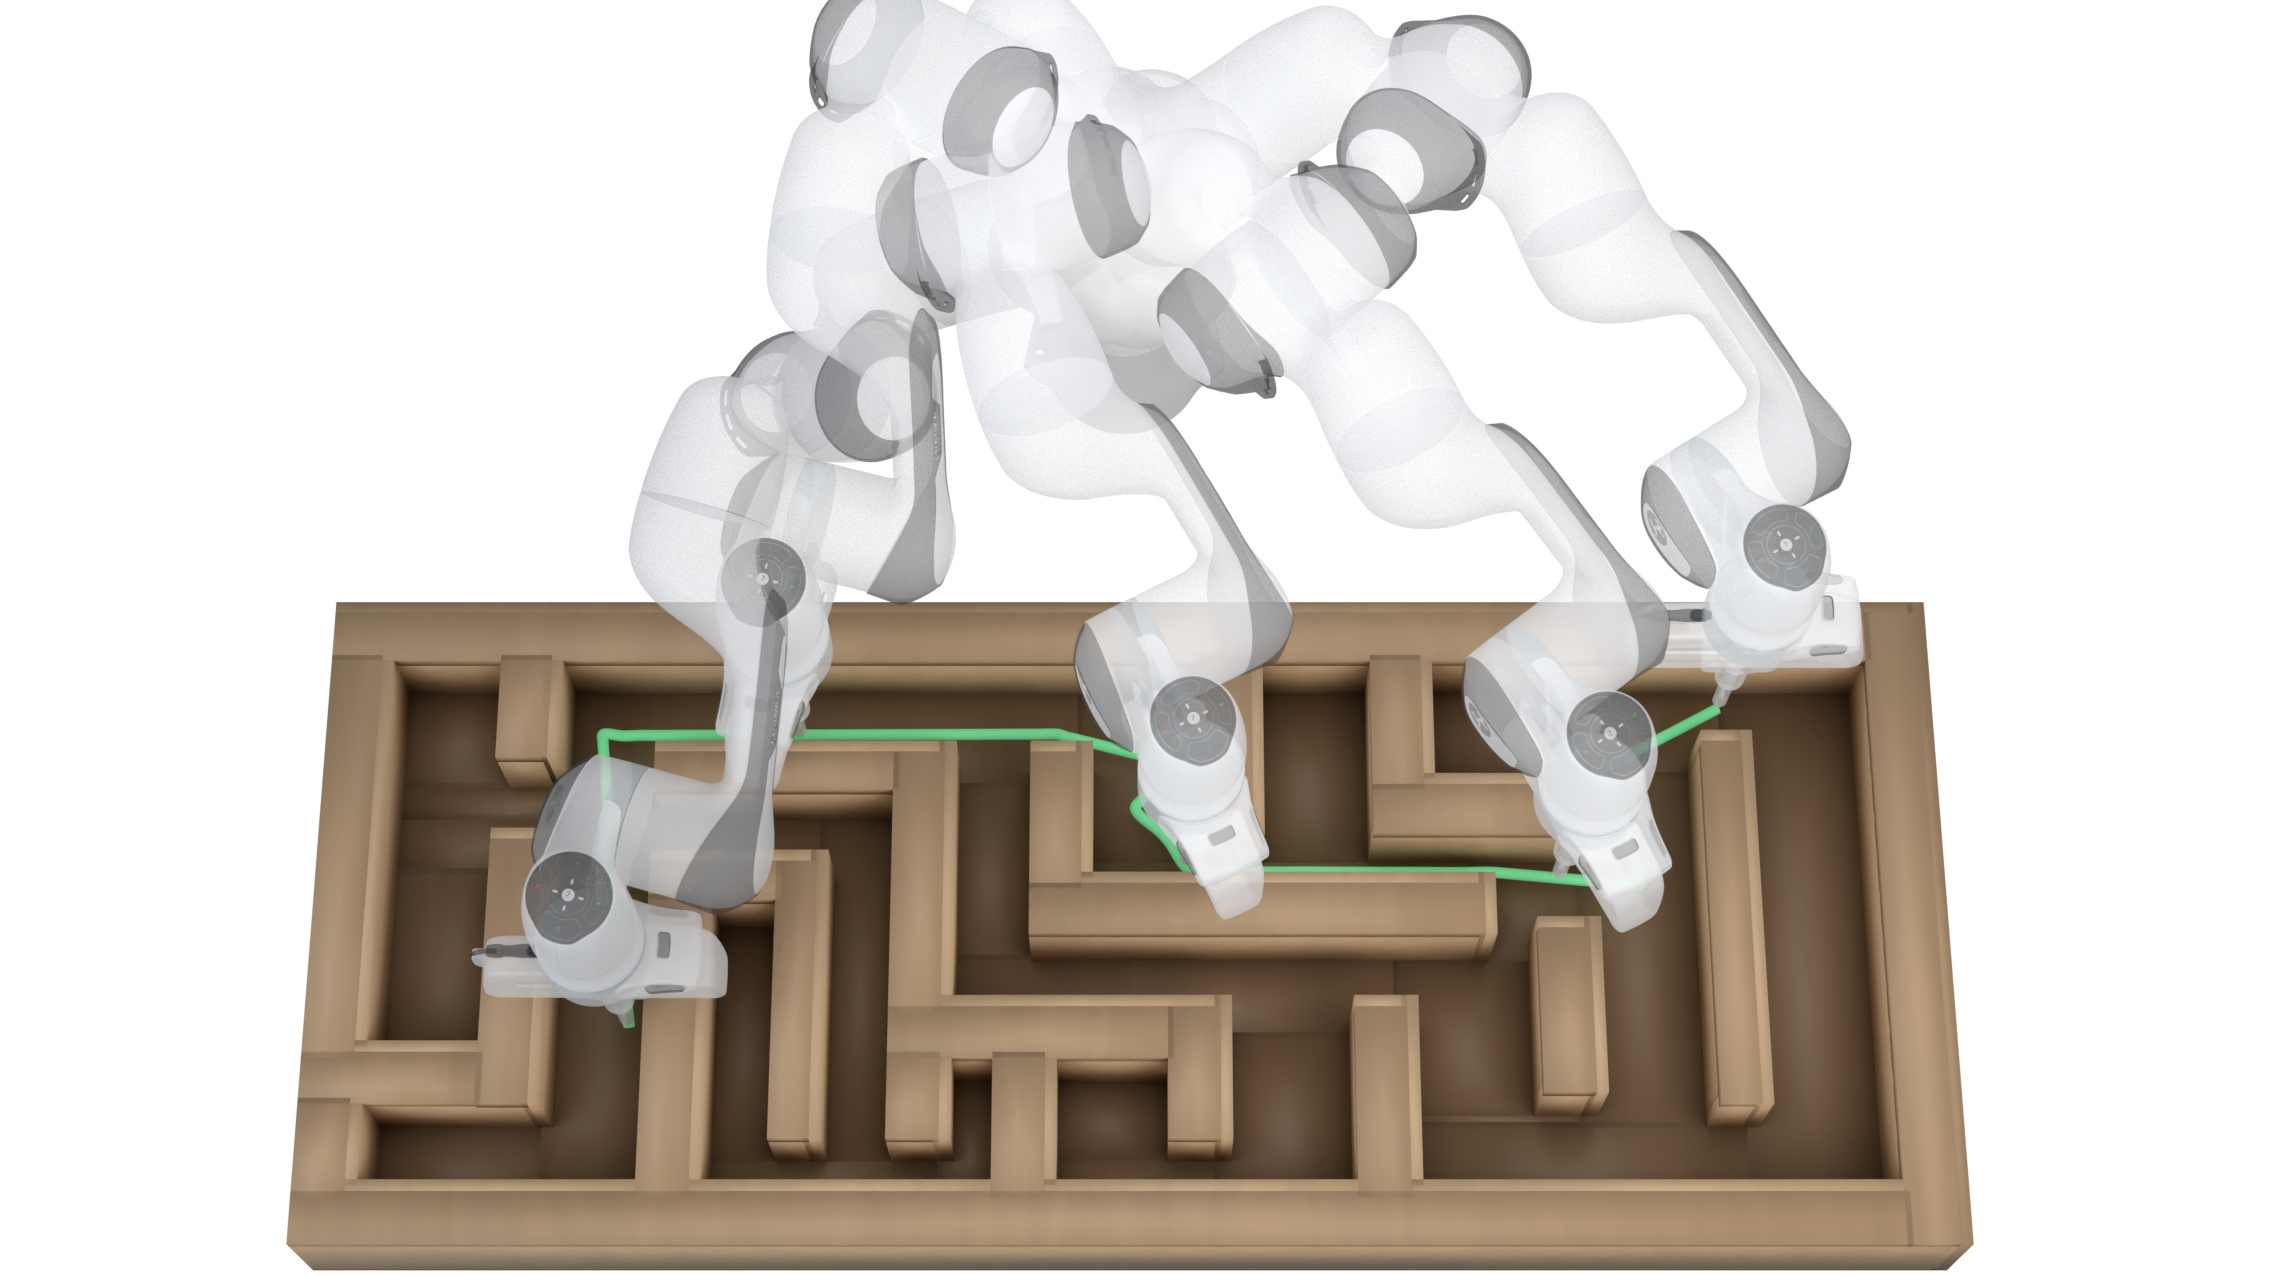
\includegraphics[width=\linewidth]{images/hero_ghosts.jpg}\par
    \captionof{figure}{Example of a solved trajectory in the maze.}
    \label{fig:maze_hero}
\end{minipage}
\end{figure*}

\section{Experimental Evaluation}
\label{sec:expts}
We evaluate our planner across different robots, with increasing DoF, and constraint complexity. All methods were evaluated on the same set of problems on a 5.4GHz Intel i7-13700K CPU with 64GB of RAM, unless specified otherwise. Each experiment highlights a distinct benefit of the planner and its potential implications. For the FR3 with a plane constraint, we show that planning on $SE(2)$ provides better scaling and strict constraint satisfaction. Through the bimanual 14-DoF Iiwa, we demonstrate the benefits of choosing the right parameterization, and the planner's high per-iteration throughput. Finally, on the RB-Y1 bimanual mobile manipulator, we show how the increased throughput can structurally change sequential planning pipelines. 

% \begin{table}[t]
% \centering\scriptsize
% \caption{Parameterizations used in each experiment.}
% \begin{tabular}{lccl}
% \toprule
% Robot & DoF & $\mathbb{P}$ & Parameterization $\Phi$ \\
% \midrule
% FR3 (maze)        & 7  & 7  & $(X,\psi)\mapsto q$, $X\in SE(3)$ \\
% Iiwa (Leader-Follower) & 14 & 8  & $(q_l,\psi_r)\mapsto(q_l,q_r)$ \\
% Iiwa (Dual-Follower)   & 14 & 8  & $({}^W\!X^B,\psi_l,\psi_r)\mapsto(q_l,q_r)$ \\
% RB-Y1 (Dual-Follower)  & 20 & 14 & $(q_\text{tor},{}^W\!X^B,\psi_l,\psi_r)\mapsto(q_\text{tor},q_l,q_r)$ \\
% \bottomrule
% \end{tabular}
% \label{tab:param_summary}
% \end{table}


% \sicomment{For maze: better scaling, failure time, easier problem-specification, strict constraint satisfaction. For iiwa, --> per-iteration planning time much lower, and how the right reparameterization can reduce planning iterations. For ruby, harder constraints and structural pipeline change}

\subsection{Task Space Constraint for the 7-DoF FR3}




% \begin{figure}
%     \centering
%     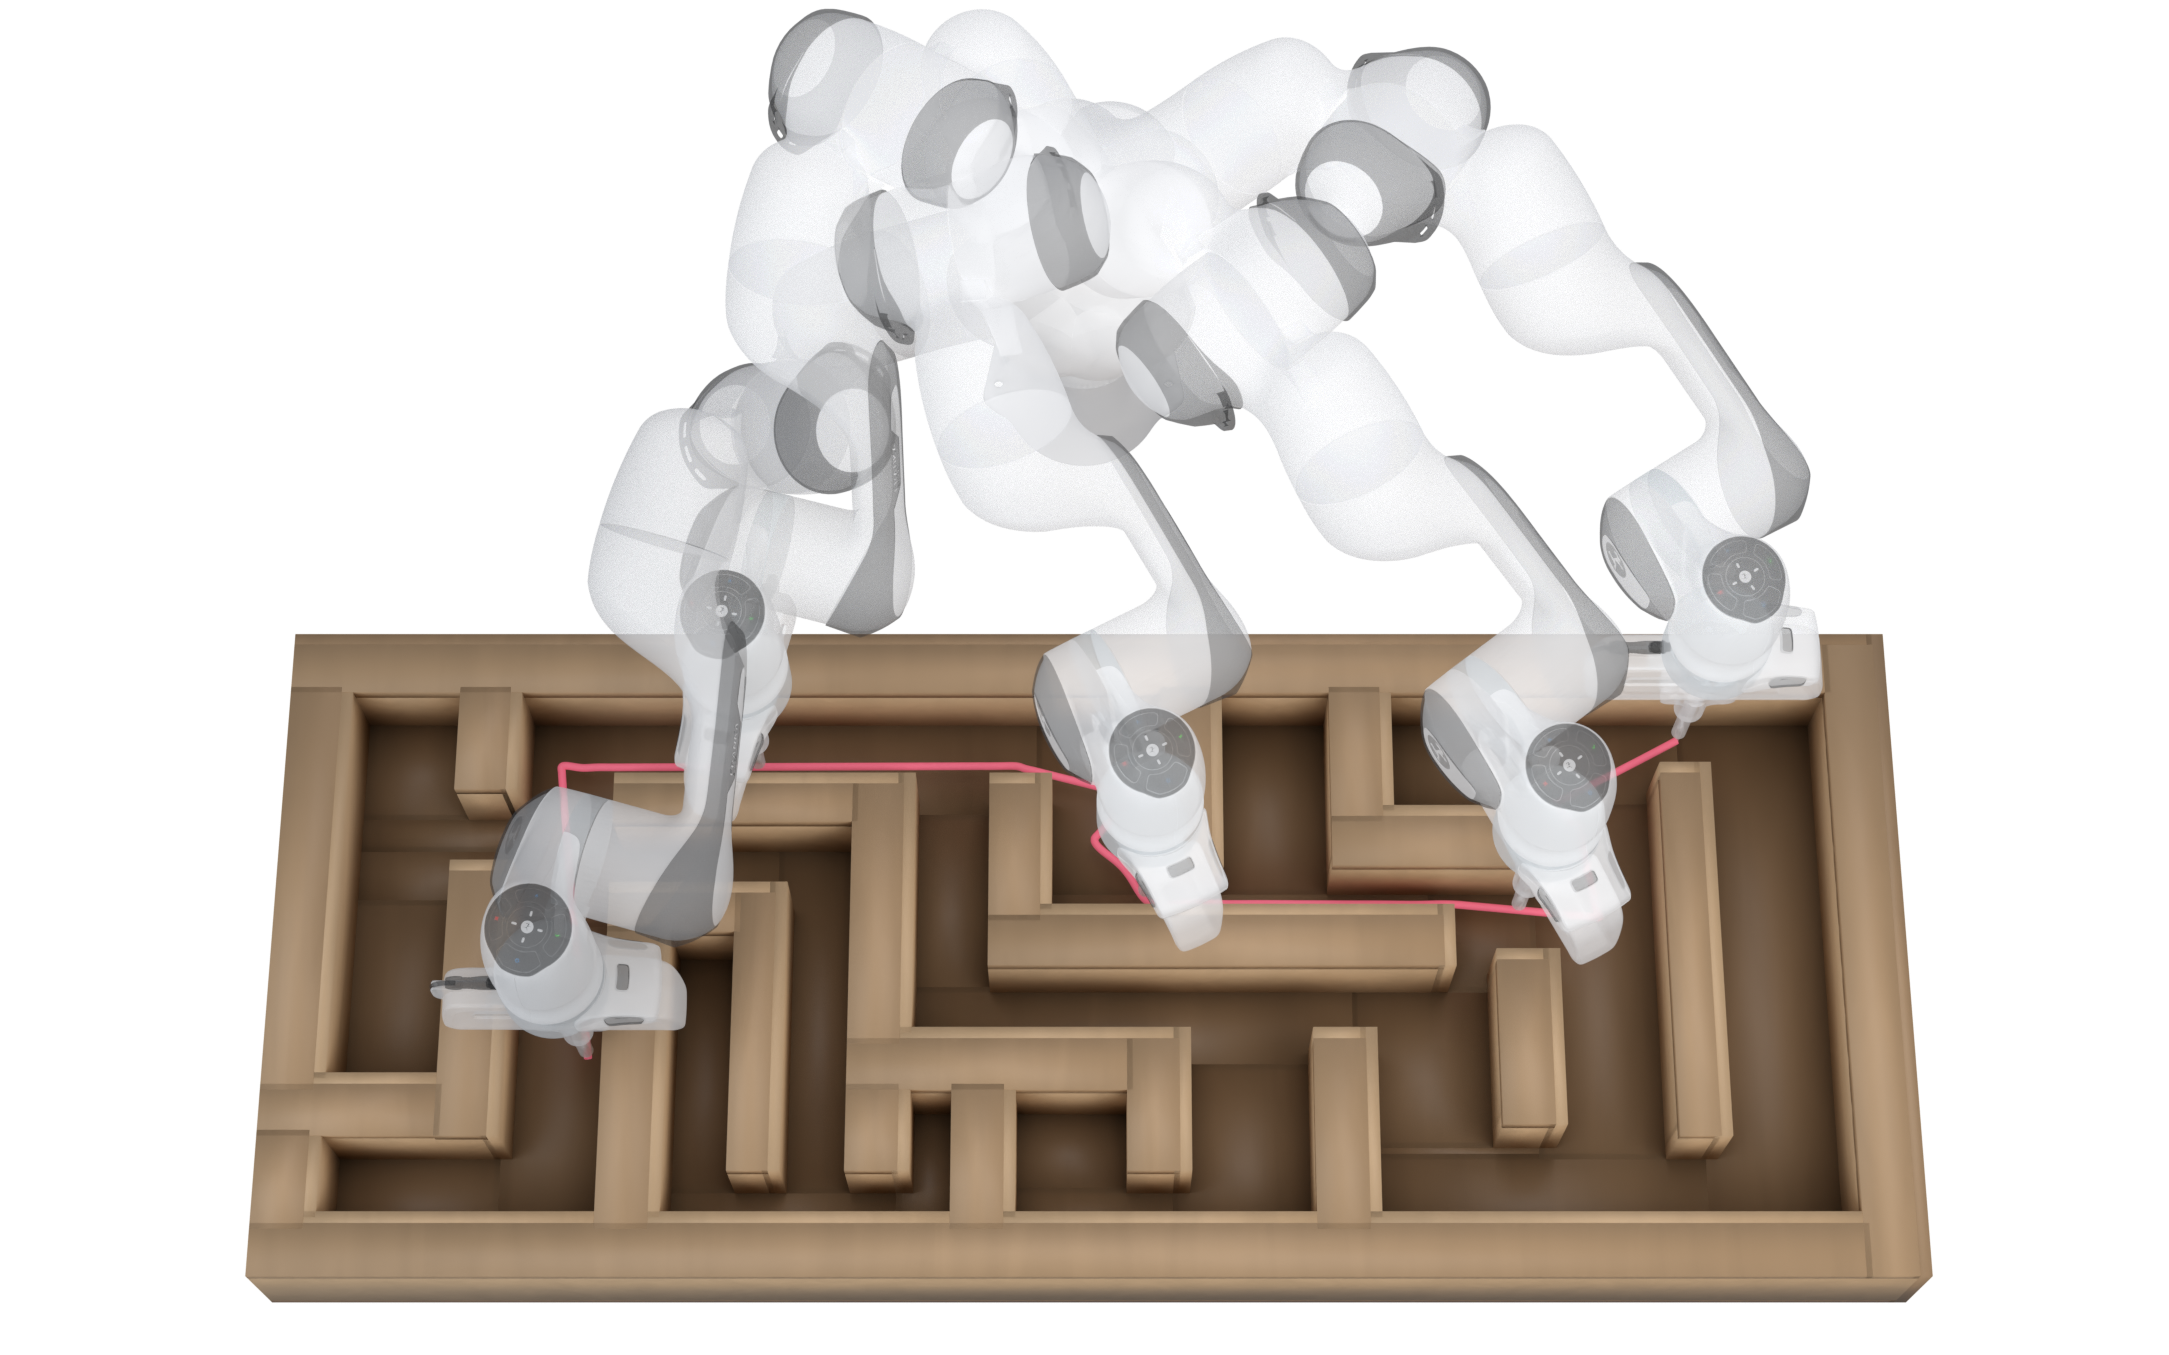
\includegraphics[width=0.99\linewidth]{images/hero_maze.png}
%     \caption{Example of a solved trajectory in the maze.}
%     \label{fig:maze_hero}
%     \vspace{-1em}
% \end{figure}


% \begin{figure}
%     \centering
%     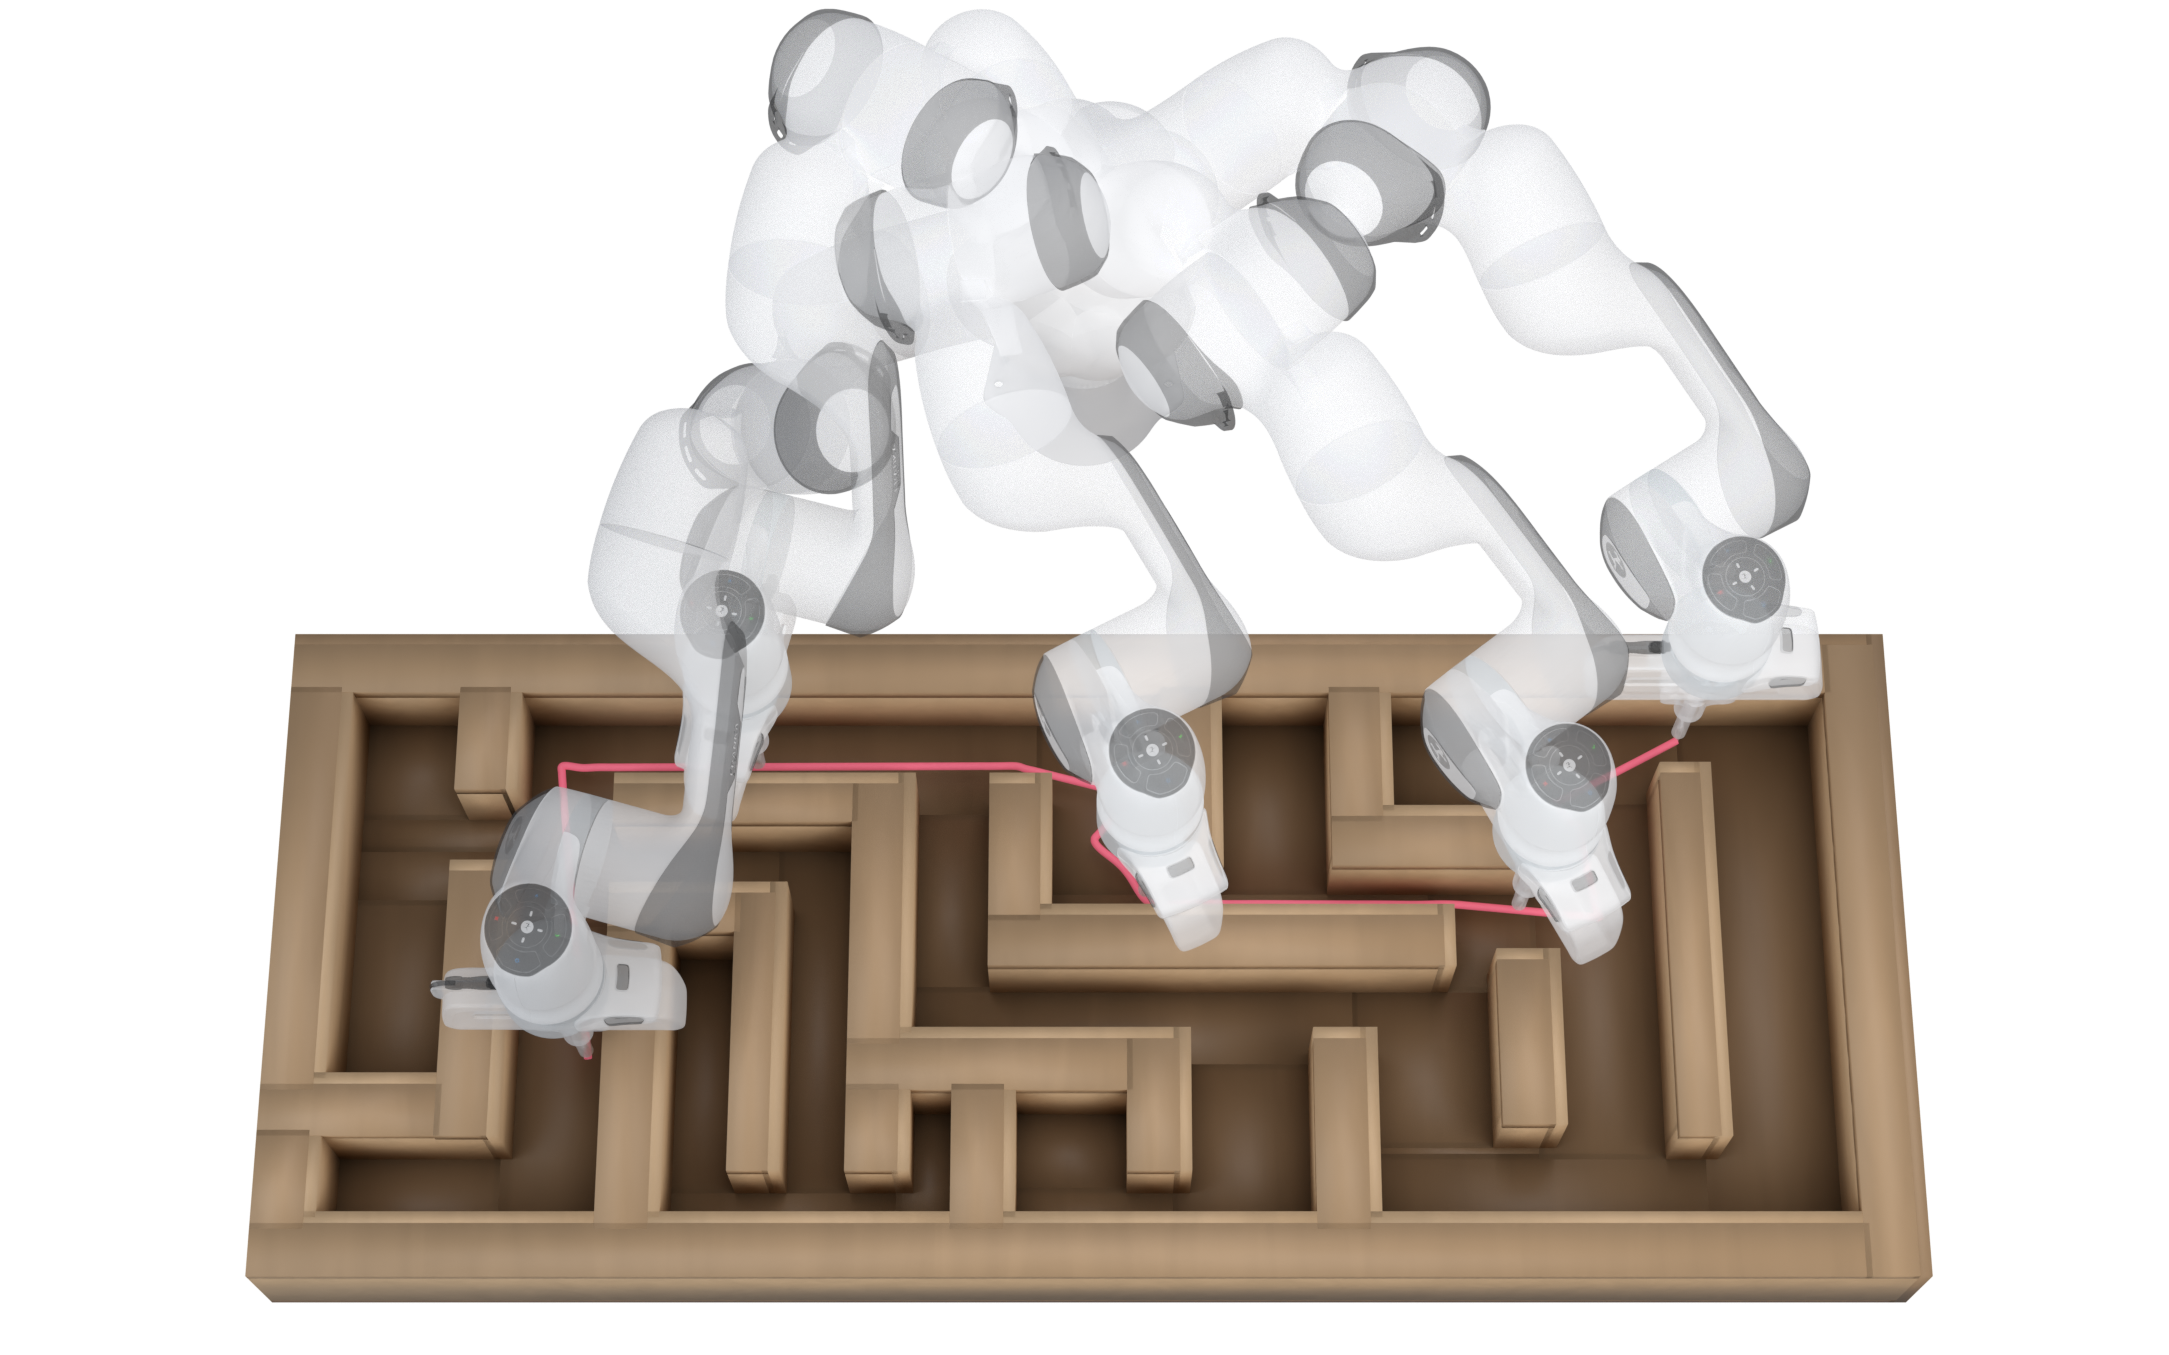
\includegraphics[width=0.95\linewidth]{images/hero_maze.png}
%     \vspace{0.5em}
%     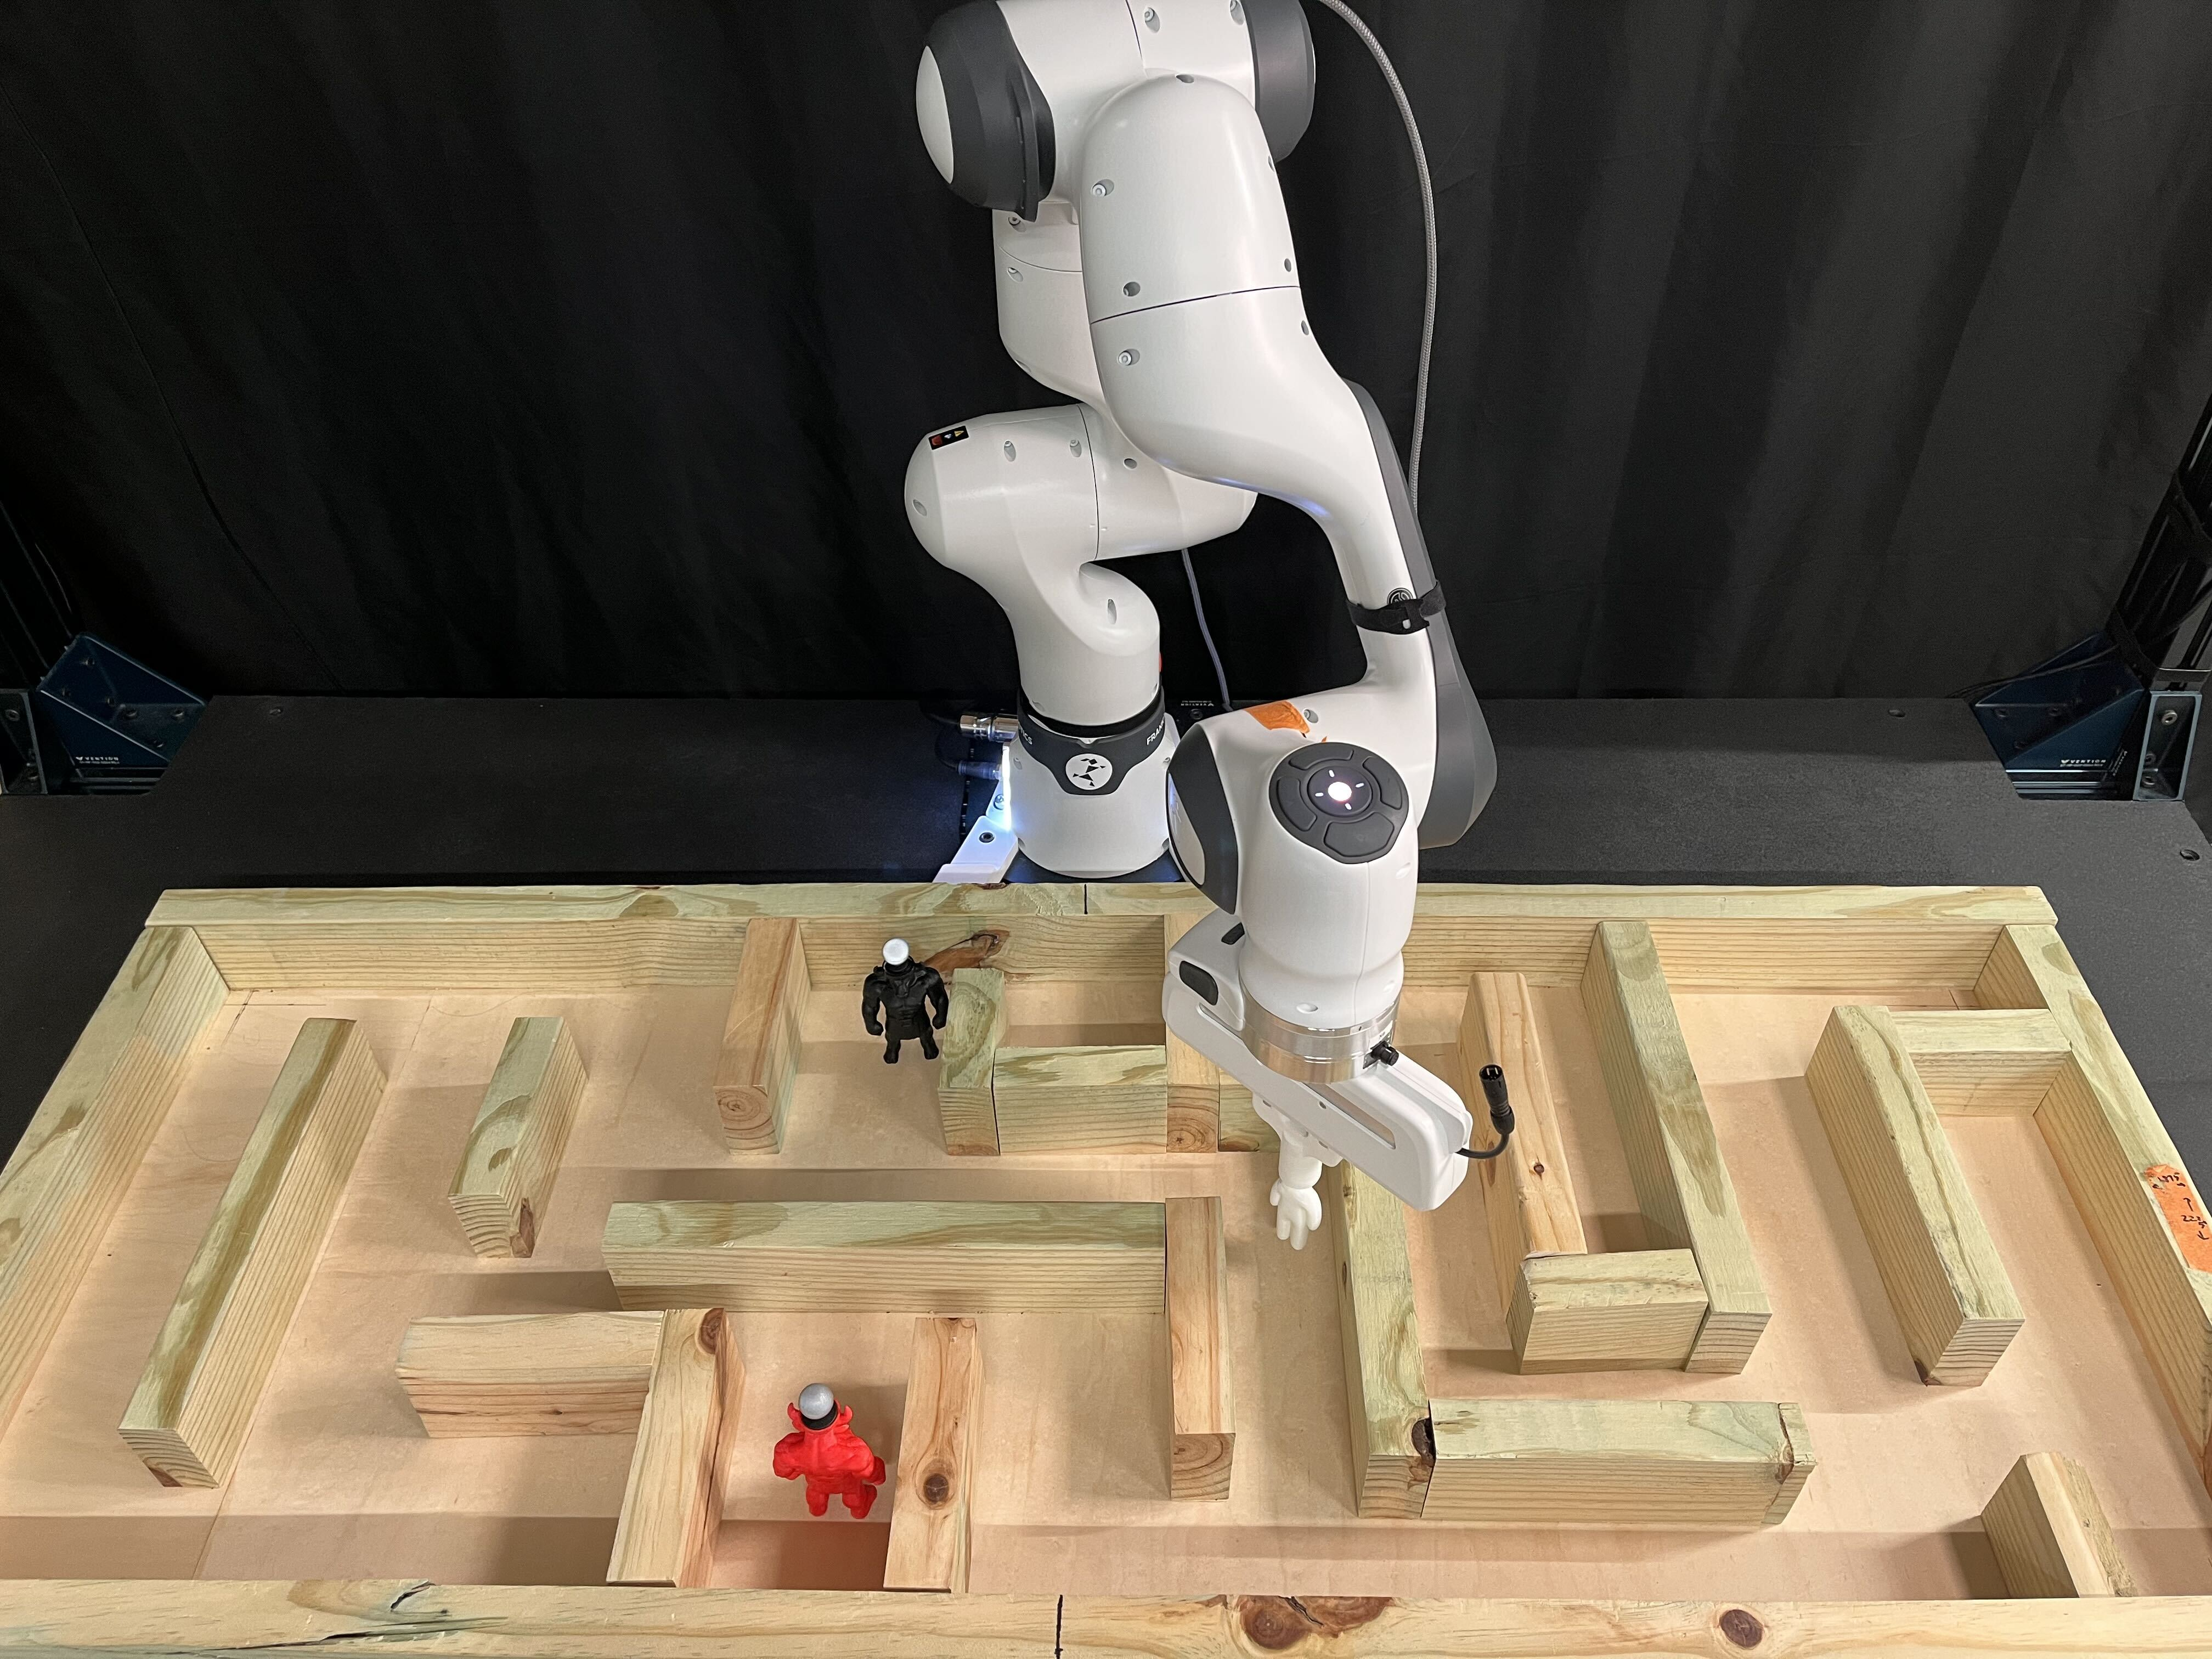
\includegraphics[width=0.75\linewidth]{images/realmaze.jpg}
%     \caption{Example of solved trajectories in the maze.}
%     \label{fig:maze_hero}
%     \vspace{-1em}
% \end{figure}


We first explore the task-space parameterization for the 7-DoF FR3 arm navigating a maze, with the end-effector constrained to the floor of the maze and its roll and pitch locked. We use the IK implementation provided by He. et al.~\cite{franka_ik2021}. It produces solutions in 4 different IK branches, with the angle of one joint used as the redundancy parameter $\psi$. Given a pose $X \in SE(3)$, $\psi \in [-\pi, \pi]$, and the desired branch $b$, it returns the configuration $q = \IK_b(X, \psi)$. The parameterized space is thus $\mathbb{P} = SE(3) \times \Psi$, which is 7-dimensional, with
\[
    \Phi : (X, \psi) \mapsto q.
\]

For the maze problem, $X$ is effectively reduced to sampling from $SE(2)$ since $z$, roll and pitch are fixed. To navigate from start to goal, it has to necessarily solve the maze. We generate 200 collision-free start-goal pairs belonging to the same SMM (such that they are sufficiently far apart). We compare it to the projection based McVAMP~\cite{iyer2026vectorizing} accelerated with the VAMP backend. We additionally ablate the early EEF collision checking (\cref{algline:pe:eefprefilter}), by disabling it in method "ReVAMP w/o EECC". Queries are terminated after 100k iterations without a solution. In addition to planning time and iterations, we record the time to resolve the $(x,y)$ goal to parameter space, and failure time.


% This is ideal for tasks constrained by the end-effector, such as tracing a line/plane, and $X$ effectively becomes the new constrained space. (for eg. if the orientation is locked, it can just be $\mathbb{R}^3$). 

% Consequently, our parameterized planning space $X$ is now $SE(2)$ with the range of $x$ and $y$ set to $\pm1m$ 
\begin{figure}[h]
\centering
\begin{subfigure}[b]{0.75\linewidth}
    \centering
    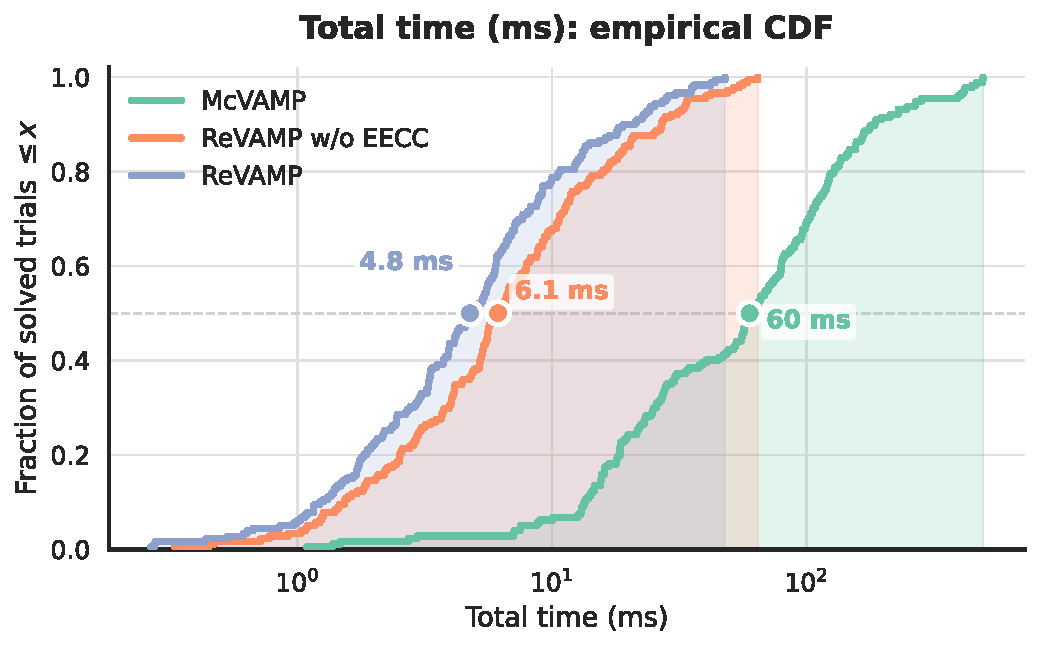
\includegraphics[width=\linewidth]{images/plots/maze/total_time_ecdf.pdf}
    \caption{Total planning time (planning + shortcutting)}
    \vspace{0.5em}
    \label{tab:maze_time}
\end{subfigure}

\begin{subfigure}[b]{0.85\linewidth}
    \centering
    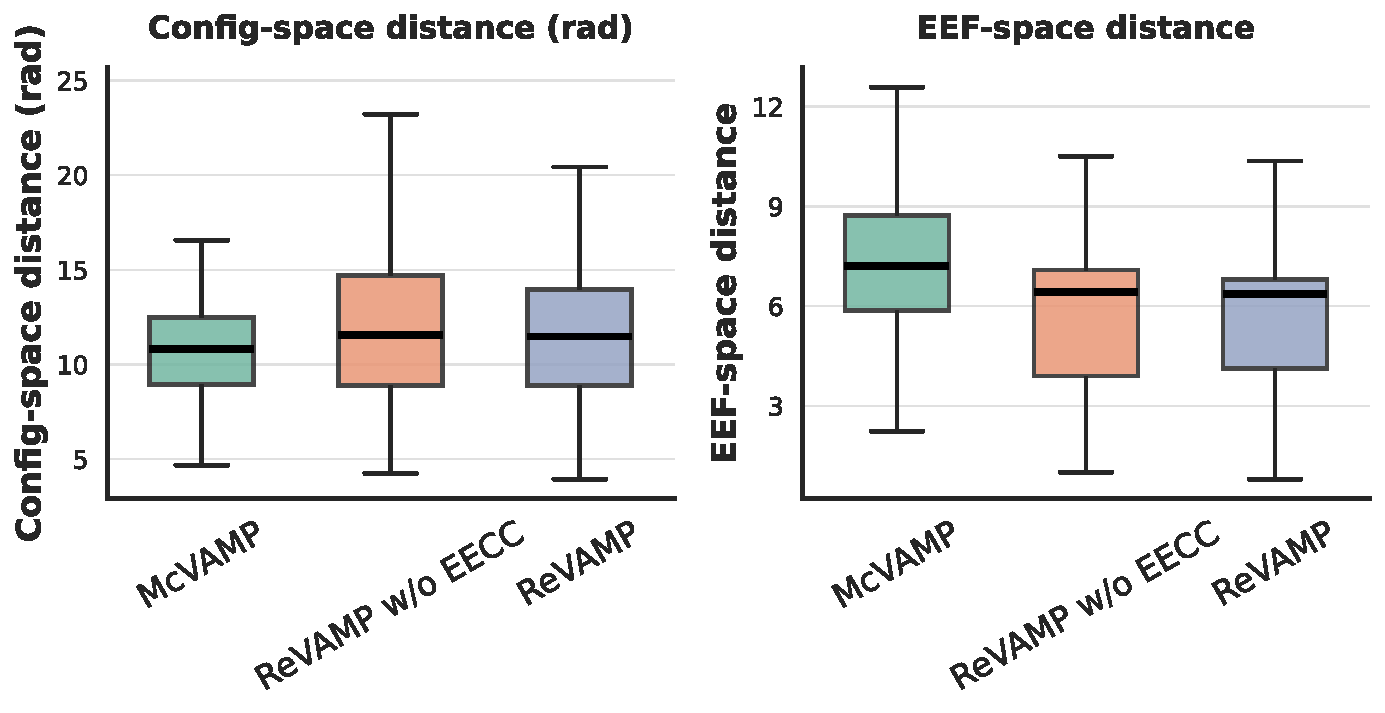
\includegraphics[width=\linewidth]{images/plots/maze/config_distance_and_eef_distance.pdf}
    \caption{Config and EEF space distance}
    \label{tab:maze_distance}
\end{subfigure}
\caption{Maze solver results: (a) planning times to solve the maze (b) Task-space and configuration space distance}
\label{tab:maze_results}
\vspace{-1em}
\end{figure}


The results in ~\cref{tab:sim_maze_results} show that ReVAMP is better suited to the problem, with better planning times without sacrificing success. It scales better with harder problems, indicated by the long-tail planning times and a $10\times$ lower failure time. This strongly supports our hypothesis that the fixed non-iterative procedure allows failed queries to terminate much earlier. 
% Since McVAMP and ReVAMP plan in configuration and end-effector space, respectively, each produces a shorter path in its corresponding planning space. 
ReVAMP also requires only $(x,y)$ start-goal queries, while McVAMP requires constraint-satisfying configurations as start-goal states. \tccomment{Don't think you've discussed this yet?} The ablation shows the benefit of early collision checking: 91.6\% of edges are rejected before computing IK, reducing latency. Nonetheless, ReVAMP without this prefilter remains faster than McVAMP, indicating most of the gain comes from the reparameterization.
% since its instruction set per-iteration is fixed. The failure time is also $10\times$ lower for the same number of iterations.


% For the maze, most of the collisions typically are between the end-effector and the environment. With this parameterization for an edge-check, EEF colliding edges can be invalidated very cheaply even before performing IK, since we sample in the task space. Empirically for the maze, \textbf{$91.6\%$} of the edges are early rejected, which produces this speed-up. While constraint-satisfying start-goal points must be provided to McVAMP for planning, PVAMP takes in start and goal end-effector points only, and resolves the SMM branch, along with the free parameter before planning, which makes planning queries easier to provide.

% McVAMP produces slightly shorter configuration distance paths, while the parameterized planner produces slightly shorter end-effector paths. This makes sense since they plan and optimize in their respective spaces. Additionally, the failure time is significantly lower for PVAMP by over $10\times$ despite an equal number of iterations, which strongly supports our hypothesis that the non-iterative procedure can help us upper-bound the planning time more easily. , since all operations within a single planning iteration are upper-bounded due to a fixed instruction set, while the projection planner needs to perform an iterative projection step that depends on the configuration's distance to the manifold
\begin{figure}
    \centering
    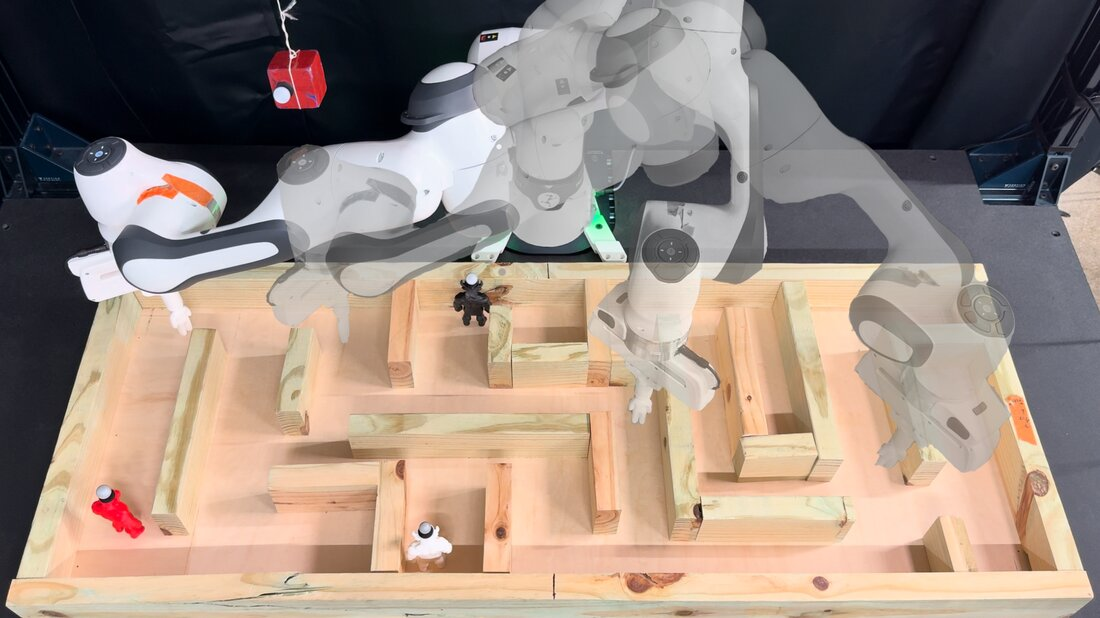
\includegraphics[width=0.95\linewidth]{images/realmazex.jpg}
    \caption{Real-world maze-setup, with obstacles that block the maze and the $C$-space. \sicomment{will try to do a ghosts in real-world, inspired by kaivalya} \tccomment{Might want to point claude at this code (overleaf comment) as an example of how to make a hardware swept volume figure.}}
    \label{fig:maze_hero_real}
    \vspace{-1em}
\end{figure}


% % Auto-generated by plot_bimanual_results.py -- paste into your LaTeX source.
% \begin{table}[!t]
% \centering
% \caption{Maze Experiment Results: Median (Mean $\pm$ std) planning times and path lengths}
% \label{tab:sim_maze_results}
% \scriptsize
% \begin{tabular}{lccc}
% \toprule
% Metric & McVAMP & ReVAMP-NoEECC & ReVAMP \\
% \midrule
% Success (\%) & 88.5 & 88.5 & \textbf{89.5} \\
% Iterations & 9442 (14644 $\pm$ 17872) & \textbf{5073 (9250 $\pm$ 13346)} & 5283 (11365 $\pm$ 17355) \\
% Resolve (ms) & -- & \textbf{0.01 (0.02 $\pm$ 0.02)} & 0.01 (0.01 $\pm$ 0.01) \\
% Planning (ms) & 46.19 (71.78 $\pm$ 92.21) & 5.35 (8.34 $\pm$ 10.49) & \textbf{4.38 (7.33 $\pm$ 8.72)} \\
% Shortcut (ms) & 12.14 (16.75 $\pm$ 13.87) & 0.60 (0.65 $\pm$ 0.38) & \textbf{0.42 (0.48 $\pm$ 0.30)} \\
% Total (ms) & 59.80 (88.53 $\pm$ 97.87) & 6.05 (8.99 $\pm$ 10.63) & \textbf{4.76 (7.81 $\pm$ 8.83)} \\
% Failure (ms) & 473.22 (463.89 $\pm$ 68.89) & 67.42 (75.88 $\pm$ 22.15) & \textbf{57.31 (60.15 $\pm$ 18.17)} \\
% Config dist. (rad) & \textbf{10.81 (10.75 $\pm$ 2.58)} & 11.80 (12.00 $\pm$ 3.65) & 11.49 (11.70 $\pm$ 3.74) \\
% EEF dist. & 7.21 (7.30 $\pm$ 2.21) & 6.40 (5.56 $\pm$ 2.09) & \textbf{6.37 (5.47 $\pm$ 2.06)} \\
% \bottomrule
% \end{tabular}
% \end{table}


% \begin{table*}[!t]
% \centering
% \caption{Median (mean $\pm$ std) planning cost and shortcut path length per method.}
% \label{tab:maze_results}
% \begin{tabular}{lccccccccc}
% \toprule
% Method & Success (\%) & Iterations & Resolve (ms) & Planning (ms) & Shortcut (ms) & Total (ms) & Failure (ms) & Config dist. (rad) & EEF dist. \\
% \midrule
% McVAMP & \textbf{93.5} &  13365 $\pm$ 20591 & -- &  68.17 $\pm$ 107.67 &  11.51 $\pm$ 11.60 &  79.68 $\pm$ 112.96 &  983.72 $\pm$ 88.72 & \textbf{ 11.81 $\pm$ 2.81} &  8.12 $\pm$ 2.47 \\
% ReVAMP & 93.0 & \textbf{ 8689 $\pm$ 15214} & \textbf{ 0.03 $\pm$ 0.02} & \textbf{ 5.77 $\pm$ 7.62} & \textbf{ 0.32 $\pm$ 0.19} & \textbf{ 6.09 $\pm$ 7.69} & \textbf{ 64.13 $\pm$ 8.79} &  13.34 $\pm$ 4.43 & \textbf{ 5.92 $\pm$ 2.04} \\
% \bottomrule
% \end{tabular}
% \end{table*}


% Auto-generated by analyze_maze_expt.py -- paste into your LaTeX source.
\begin{table}[!t]
\centering
\scriptsize
\label{tab:real_maze_results}
\vspace{1em}
\begin{tabular}{lcc}
\toprule
Metric & McVAMP & ReVAMP \\
\midrule
Success (\%) & 91.89 & \textbf{95.65} \\
Planned z-error (mm) & 1.020 (1.227 $\pm$ 0.988) & \textbf{0.000 (0.000 $\pm$ 0.000)} \\
Executed z-error (mm) & 1.075 (1.307 $\pm$ 0.966) & \textbf{0.191 (0.221 $\pm$ 0.168)} \\
Plan. time (ms) & 146.19 (500.90 $\pm$ 666.05) & \textbf{11.95 (37.72 $\pm$ 67.07)} \\
Iterations & 10292 (30745 $\pm$ 39038) & \textbf{4570 (11930 $\pm$ 17295)} \\
\bottomrule
\end{tabular}
\caption{Real-Maze results. Values are median (mean $\pm$ std).}
\end{table}


We next evaluate the planners' validity in the real world, using the same maze setup~\cref{fig:maze_hero_real}, but with dynamic obstacles that block parts of the maze and the robot configuration space. The system must replan whenever the environment changes. We run both planners for approximately $60$s on an RTOS with a 2.5~GHz Intel i5-6500T CPU and 8~GB RAM, recording planning statistics and the executed joint trajectory at 30~Hz. We perform FK on the recorded states and measure the end-effector's deviation from the desired maze plane. \cref{tab:real_maze_results} clearly shows the benefits of our planner on a resource-constrained system. Beyond order-of-magnitude faster planning times, it importantly adheres to the task-constraint strictly. The planned trajectory remains on the desired plane, and the executed trajectory deviates by only $0.2$~mm on average (due to controller error).

% In addition, it is also clear  Interestingly, this also produces much shorter end-effector and configuration paths, which probably indicates that the landscape of this space is perhaps not as warped as the projection planner. Despite being restricted to a single c-bundle, it is able to solve a similar number of problems as well. 


% Show the maze problem, describe the constraint here
% Problem generation: Key -- both start and goal are on the same GCP branch!


% \begin{tabular}{c|c|c|c|c|c|c|}
% Method & SuccessRate & Planning Time & EEF Distance & Config Distance & Failure-cases time & Shortcutting Time \\
% PVAMP  & & & & &  \\
% McVAMP  & & & & &
% \end{tabular}

% 3 axes of results

% start with maze
% - you can do early rejection which is a good benefit → exploit task-space properties
% - Bounded planning time —> show worst case planning times, and show shortcutting time to indicate it is a trivial operation
% - respect constraints at every single point, which is a benefit
% clear speedup over parameterized. harder problems require more iterations

\subsection{Bimanual Constraint for the 14-DoF Bimanual Iiwa}


% For the 14-DoF KUKA Iiwa dual arm, we use the smooth IK solution proposed by \cite{cohn2024constrained} for each arm. 
We next test the system on a more complex constraint for a higher DoF system, the Bimanual 14-DoF Iiwa robot arms. Here, the relative pose between the end-effectors of the two arms is fixed (to the dimensions of the object it transports) throughout the motion. Given configurations $q_l$ and $q_r$ for the left and the right arms, and a fixed relative transform $\monogram{X}{l}{r}$ between the end-effectors, the constraint is $\FK(q_l)^{-1}\,\FK(q_r) = \monogram{X}{l}{r}$ . \tccomment{Might need to cite Russ' textbook for monogram notation (see comment for link).} We use the smooth IK solution proposed by Cohn et al. \cite{cohn2024constrained} for each arm and study two parameterizations built on it.

\paragraph{Leader-Follower Setup}
This is identical to the parameterization used by ~\cite{cohn2024constrained}: the leader arm samples in its configuration space $C_l$, while the follower arm's configuration is derived from the leader's end-effector pose, $q_r = \IK_b\!\left(\FK(q_l)\,{}^{l}X^{r}, \psi_r\right)$.
% \tccomment{I'm wary of taking credit for leader-follower since many others have used it before -- suggest ``used by'' instead of ``proposed by''?}
% The compiler produces the instruction set for the entire operation. 
The parameterized space is therefore $\mathbb{P} = C_l \times \Psi$, where $q_l \in C_l$ is the leader's configuration and $\psi_r$ is the follower's free parameter. The 14-DoF configuration space is reduced to an \textbf{8-D} space, with the follower arm locked to a specified SMM branch. 
\[
    \Phi : (q_l, \psi_r) \mapsto (q_l, q_r).
\]

\paragraph{Dual-Follower Setup}
Given the object pose $\monogram{X}{W}{B}$, fixed grasp transforms ${}^{B}X^{l}$ and ${}^{B}X^{r}$, and $\psi_l$ and $\psi_r$ for each arm, we compute the desired end-effector pose of each arm, ${}^{W}X^{B}\,{}^{B}X^{l}$ and ${}^{W}X^{B}\,{}^{B}X^{r}$, and resolve both independently with $\IK_b$. The resulting space is $\mathbb{P} = SE(3) \times \Psi \times \Psi$, also an \textbf{8-D} parameterized space. Unlike the Leader-Follower setup, both arms are now locked to a single branch, which reduces the solution space. This is nevertheless desirable for tasks with additional constraints, such as keeping the box upright.
\[
    \Phi : ({}^{W}X^{B}, \psi_l, \psi_r) \mapsto (q_l, q_r).
\]

% \begin{figure}[h]
% \centering
% \begin{subfigure}[b]{0.75\linewidth}
%     \centering
%     \includesvg[width=\linewidth]{images/plots/bimanual/bim_total_time_ecdf.svg}
%     \caption{Total planning time (planning + shortcutting)}
%     \label{fig:bimanual_time}
% \end{subfigure}

% \begin{subfigure}[b]{0.85\linewidth}
%     \centering
%     \includesvg[width=\linewidth]{images/plots/bimanual/bim_config_distance_and_eef_distance.svg}
%     \caption{Config and EEF space distance}
%     \label{fig:bimanual_distance}
% \end{subfigure}
% % \vspace{0.5em}
% \caption{Bimanual traverse results: (a) planning times (b) Task-space and configuration space distance \tccomment{Make sure to be consistent on the terminology for two followers (used ``Task-Space IK'' in previous section)}}
% \label{fig:bimanual_results}
% \vspace{-1em}
% \end{figure}

\begin{figure}[h]
\centering
\begin{subfigure}[b]{0.75\linewidth}
    \centering
    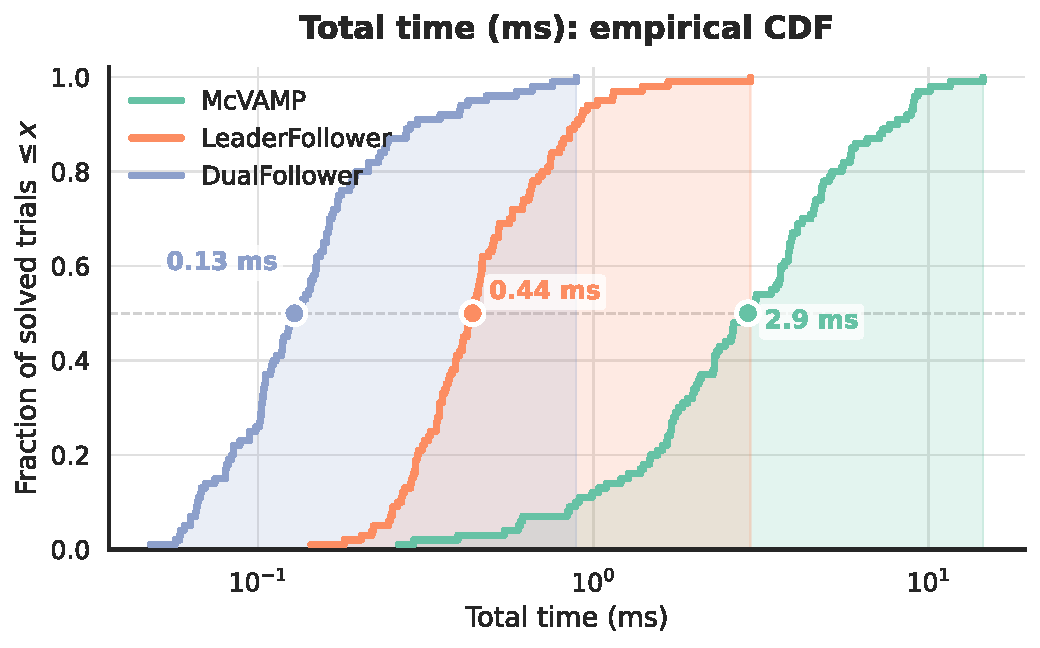
\includegraphics[width=\linewidth]{images/plots/bimanual/bim_total_time_ecdf.pdf}
    \caption{Total planning time (planning + shortcutting)}
    \vspace{0.5em}
    \label{fig:bimanual_time}
\end{subfigure}

\begin{subfigure}[b]{0.85\linewidth}
    \centering
    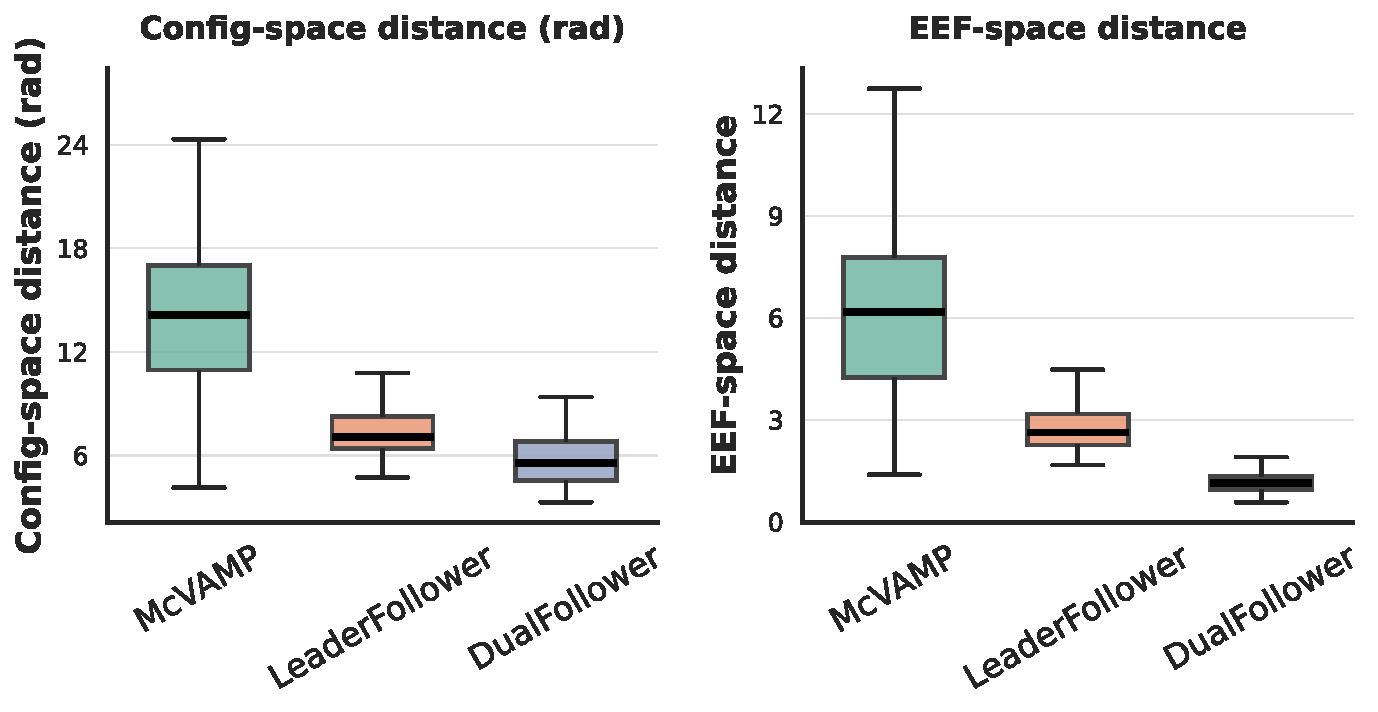
\includegraphics[width=\linewidth]{images/plots/bimanual/bim_config_distance_and_eef_distance.pdf}
    \caption{Config and EEF space distance}
    \label{fig:bimanual_distance}
\end{subfigure}
\caption{Bimanual transport results: (a) planning times (b) Task-space and configuration space distance \tccomment{Make sure to be consistent on the terminology for two followers (used ``Task-Space IK'' in previous section)}}

\label{fig:bimanual_results}
\vspace{-1em}
\end{figure}


\begin{table*}[!t]
\centering
\scriptsize
% \footnotesize
\vspace{0.2em}
\begin{tabular}{lcccccc}                                                                                                               \toprule
Method & Iterations & Planning (ms) & Shortcut (ms) & Total (ms) & Config dist. (rad) & EEF dist. \\       
\midrule
\textbf{\textcolor[HTML]{66C2A5}{McVAMP}} & 310 (437 $\pm$ 358) & 2.80 (3.56 $\pm$ 2.68) & 0.02 (0.07 $\pm$ 0.14) & 2.89 (3.63 $\pm$ 2.73) & 14.12 (14.03 $\pm$ 4.67) & 6.17 (6.22 $\pm$ 2.45) \\
\textbf{\textcolor[HTML]{FC8D62}{LeaderFollower}} & 1618 (2249 $\pm$ 2057) & 0.36 (0.45 $\pm$ 0.35) & 0.08 (0.09 $\pm$ 0.04) & 0.44 (0.53 $\pm$ 0.36) & 7.06 (7.30 $\pm$ 1.37) & 2.63 (2.77 $\pm$ 0.71) \\
\textbf{\textcolor[HTML]{8DA0CB}{DualFollower}} & \textbf{58 (75 $\pm$ 68)} & \textbf{0.11 (0.15 $\pm$ 0.13)} & \textbf{0.02 (0.02 $\pm$ 0.02)} & \textbf{0.13 (0.17 $\pm$ 0.14)} & \textbf{5.54 (5.68 $\pm$ 1.50)} & \textbf{1.14 (1.17 $\pm$ 0.32)} \\
\bottomrule
\end{tabular}
\caption{Median (mean $\pm$ std) planning cost and shortcut path length per method.}
\label{tab:bimanual_results_tab}
\end{table*}


We use the same problem set proposed by ~\cite{cohn2024constrained} between three fixed positions, with 200 trials, randomizing the start-goal pairs. ~\cref{tab:bimanual_results_tab} compares McVAMP with the Leader-Follower and Dual-Follower parameterizations. From the results in~\cref{tab:bimanual_results_tab}, it is clear that the parameterized planners achieve a significantly lower per-iteration planning time, particularly evident for the LeaderFollower. It is $6\times$ faster than McVAMP despite taking $5\times$ more iterations. This suggests that the parameterized planner scales much better with the dimensionality and the constraint complexity. Both planners also show lower planning times and trajectory distances. 
Interestingly, the Dual-Follower parameterization outperforms the Leader-Follower across all metrics. This is likely because all start-goal pairs lie in the same SMM for both arms, making the problem easier. Beyond vectorization, this experiment demonstrates that choosing the right planning space can significantly reduce the planning iterations, making the problem easier to solve in the new space.
% The projection planner on the other hand has a slightly better shortcutting time. This is probably because most of the configurations in a straight-line between two configurations in the planned trajectory already lie on the constraint manifold, hence there is minimal effort needed to project them.

% \begin{tabular}{c|c|c|c|c|c|c|}
% Method & SuccessRate & Planning Time & EEF Distance & Config Distance & Failure-cases time & Shortcutting Time \\
% PVAMP-LeaderFollower  & & & & &  \\
% PVAMP-TaskSpace  & & & & & \\
% McVAMP  & & & & & &
% \end{tabular}


% Go to bimanual iiwa planner
% - per-iteration cost is significantly lower
% - Maybe even show IK is faster

\subsection{Pick and Place for RB-Y1}
\label{expts:ruby}
Our final experiment deploys our planner to generate whole-body motions for a full pick-and-place pipeline on the Rainbow Robotics RB-Y1 mobile manipulator. We use the parameterization based on the Inverse Function Theorem (IFT) work proposed by~\cite{cohn2026planning} . With a slight abuse of terminology, for the rest of the discussion, we refer to the entire pick-and-place pipeline method used by the work as IFT. It has two 7-DoF arms attached to a 6-DoF torso, and a wheeled base. Since we are evaluating a pure manipulation task, we disable the wheels, and fix the base at origin, which makes it a 20-DoF system. Again, the goal is a bimanual-constrained box-transport task, whose constraints are similar to the 14-DoF Iiwa arm. The robot must pick up a box from the floor with both hands and place it on a table next to the robot. It must also satisfy a stability constraint requiring the center of mass (CoM) to remain within the support polygon.

% For the purposes of this setup, we fix the base to be at (0, 0, 0) and allow the other joints to move. 

We use IKFast~\cite{ikfast} to generate the IK solution for each arm, and compile them as described in~\cref{sec:compileik}.
The arms each have 8 disconnected self-motion manifolds, with redundancy $\psi$ parameterized by the angle of the $3$rd joint.
% \tccomment{Using ``branchless code'' in one sentence and talking about ``IK solution branches'' immediately after is confusing. Unfortunate overlapping terminology, but maybe ``The RB-Y1 arms have 8 disconnected self-motion manifolds, with redundancy parameterized by the angle of the $n$th joint (don't remember which).''}
% Similar to the bimanual iiwa, we implement a Dual-Follower IK setup. Given the torso joints, a mid-pose and a desired transform between the two arms, $T \in SE(3)$, the compiled instruction set first computes the goal pose of each arm, which is then passed through the respective per-arm IK mappings to obtain the desired configuration, while retaining the base and torso joints. 
We implement a Dual-Follower parameterization: the torso joint configuration, the held box pose, and free parameters $\psi_l$ and $\psi_r$ for each arm define a 14-DoF space,
\[
    \Phi : (q_\text{torso}, {}^{W}X^{B}, \psi_l, \psi_r) \mapsto (q_\text{torso}, q_l, q_r),
\]
where $B$ is the box frame.
% When carrying the box, we use the parameterization defined in~\cref{sec:rubyarms}
% \[
%     \Phi : (q_\text{torso}, {}^{W}X^{B}, \psi_l, \psi_r) \mapsto (q_\text{torso}, q_l, q_r),
% \]
% where $B$ is the box frame and $\psi_{left}$ and $\psi_{right}$ are the arms' respective self-motion parameters.
As with IFT, we test 20 box poses in a 4-by-5 grid (3cm apart) on the floor in front of the robot. This experiment demonstrates the scaling of our method along multiple axes. The constrained problem has only 0.012\% of its parameterized space feasible under collision and stability constraints (an inequality constraint defined by support polytopes), as opposed to the 33.1\% of the C-space available for unconstrained planning. 


% The high dimensionality of the system -- 20-DoF for unconstrained motions and 14-DoF for the constrained motions -- is a classic challenge for sampling-based planning.
% Besides collision avoidance, we must ensure  stability: a significant portion of the robot's mass is concentrated in the torso and arms, so the risk of falling over when picking up the box from the floor is a major hazard.
% This appears as a complicated nonlinear inequality constraint (the center of mass must be over the support polytope [cite SHR]), further reducing the measure of the free space.
% While 33.1\% of C-Space is feasible for the unconstrained plans, only 0.012\% of the parameterized space is feasible for the constrained plans.

We retain the complete planning pipeline from IFT~\cite{cohn2026planning}, which at a high level includes: (1) optimization IK for the pick, carry, and place poses, (2) unconstrained plan from start-to-pre-pick configuration, and place-to-home configuration, (3) constrained motions for pick to carry waypoint followed by carry to place and (4) trajectory optimization to improve the plan and TOPPRA for time parameterization.

% At a high level, we use the following pipeline:
% \begin{enumerate}
%     \item Optimization IK to compute pick, carry, and place poses.
%     \item Unconstrained motion from the start configuration to a pre-pick configuration, followed by a short motion from pre-pick to the pick itself.
%     \item Constrained motion from the pick configuration to a carrying configuration.
%     \item Constrained motion from the carrying configuration to a place configuration.
%     \item A short unconstrained motion from the place configuration to a post-place configuration, followed by a larger motion back to the start.
% \end{enumerate}
% Both unconstrained and constrained motions use BiRRT plus shortcutting to generate an initial guess, trajectory optimization to improve upon the initial guess, and TOPPRA to determine the fastest time parameterization of the trajectory that obeys joint limits.
% (The short pick and place motions heuristically try a straight-line motion in C-space first.)
We differ from IFT in two significant ways.
The first change is straightforward: the use of our vectorized planner to construct initial guesses for the constrained planning legs. Second, and more significantly, we change how pick and place poses are selected. IFT generates a collection of configurations and uses problem-specific heuristics to select candidates for motion planning, with fallbacks when these candidates are not plannable.
In contrast, we solve a constrained motion planning problem between \emph{every} triple of pick, carry, and place configurations\footnote{
    This only requires solving $2n^2$ planning problems, since the plans between pick and carry are independent of the plans between carry and place.
}, and then simply select the configurations yielding the shortest plan.
This is faster, simpler, and provides better motion plans, and is wholly enabled by the incredible speed of our vectorized planner.
Additionally, to evaluate the planner's benefits, we run 20 direct pick-to-place trials without the ``carry" waypoint used in IFT, simplifying the planning problem. \tccomment{Why ``retraction''? Maybe ``waypoint''?}
% Finally, [IFT Paper] plans to a retract ``carry" point before placing it, in order to encourage easier simpler paths. With our increased throughput, we run 20 additional experiments for the same initial poses of the box, but planning directly from the pick to place position without the lift retraction, which makes the planning problem harder.
% \begin{table}[!t]
%   \centering
%   \renewcommand{\arraystretch}{0.9}
%   \caption{
%       RB-Y1 box pickup planning results over the 20-point grid.
%       Both pipelines plan all 20 points successfully and pass
%       dense feasibility checks.
%   }
%   \label{tab:ruby_results}
%   \begin{tabular*}{\columnwidth}{@{}l@{\extracolsep{\fill}}cc@{}}
%   \toprule
%   \textbf{Metric} & \textbf{Prior Pipeline} & \textbf{Ours} \\
%   \midrule
%   \multicolumn{3}{@{}l}{\textit{Time to Plan (s), mean / max}} \\
%   Median                       & 43.6 & \textbf{17.9} \\
%   Mean                         & 56.1 & \textbf{19.6} \\
%   Max                          & 135.0 & \textbf{29.9} \\
%   \midrule
%   \multicolumn{3}{@{}l}{\textit{Selected Stages (s), mean / max}} \\
%   Sampling-Based Planning      & 16.0 / 61.4 & \textbf{1.7 / 2.7} \\
%   Optimization IK              & 19.4 / 84.0 & \textbf{5.1 / 16.0} \\
%   Trajectory Opt.\ (Guess)     & 7.0 / 10.2  & \textbf{2.9 / 4.6} \\
%   Trajectory Opt.\ (Solve)     & 5.6 / 29.6  & 5.7 / 8.9 \\
%   TOPPRA                       & 5.3 / 6.3   & \textbf{1.7 / 1.8} \\
%   \midrule
%   \multicolumn{3}{@{}l}{\textit{Planned Trajectory Quality, mean / max}} \\
%   Path Length (rad)            & 18.03 / 20.67 & \textbf{17.39 / 19.17} \\
%   Duration (s)                 & 35.9 / 46.1   & \textbf{31.4 / 34.3} \\

%   \bottomrule
%   \end{tabular*}
% \end{table}


% \begin{table}[!t]
%   \centering
%   \renewcommand{\arraystretch}{0.9}
%   \caption{
%       RB-Y1 box pickup planning results over the 20-point grid, comparing ogrrt, mcvamp, task\_space.
%   }
%   \label{tab:grid_comparison}
%   \begin{tabular*}{\columnwidth}{@{}l@{\extracolsep{\fill}}ccc@{}}
%   \toprule
%   \textbf{Metric} & \textbf{ogrrt} & \textbf{mcvamp} & \textbf{task\_space} \\
%   \midrule
%   \multicolumn{4}{@{}l}{\textit{Time to Plan (s), mean / max}} \\
%   Median                       & 37.1 & 20.2 & \textbf{17.6} \\
%   Mean                         & 46.7 & 21.8 & \textbf{18.4} \\
%   Max                          & 100.0 & 34.8 & \textbf{27.9} \\
%   \midrule
%   \multicolumn{4}{@{}l}{\textit{Selected Stages (s), mean / max}} \\
%   Sampling-Based Planning      & 17.4 / 66.5 & 1.3 / 2.6 & 1.3 / 2.7 \\
%   Optimization IK              & 13.4 / 26.0 & 4.4 / 16.6 & \textbf{4.3 / 16.3} \\
%   Trajectory Opt.\ (Guess)     & 6.2 / 8.4 & 6.7 / 8.4 & \textbf{4.5 / 6.7} \\
%   Trajectory Opt.\ (Solve)     & \textbf{3.9 / 19.8} & 4.7 / 18.0 & 4.0 / 7.0 \\
%   TOPPRA                       & 3.2 / 3.5 & 1.5 / 1.5 & 1.5 / 1.5 \\
%   \midrule
%   \multicolumn{4}{@{}l}{\textit{Planned Trajectory Quality, mean / max}} \\
%   Path Length (rad)            & 17.74 / 19.46 & \textbf{17.55 / 19.35} & 17.78 / 20.43 \\
%   Duration (s)                 & 32.7 / 35.5 & \textbf{31.9 / 34.7} & 32.0 / 35.9 \\
%   \midrule
%   \multicolumn{4}{@{}l}{\textit{Constrained-Leg Path Length (rad), mean / max -- raw search vs after TrajOpt}} \\
%   Before TrajOpt (raw search)  & 6.90 / 7.88 & \textbf{5.07 / 5.91} & 7.10 / 9.33 \\
%   After TrajOpt + TOPPRA       & 6.21 / 8.13 & \textbf{5.59 / 7.21} & 5.82 / 8.29 \\
%   \bottomrule
%   \end{tabular*}
% \end{table}

% \begin{table}[!t]
%   \centering
%   \renewcommand{\arraystretch}{0.9}
%   \caption{
%       RB-Y1 box pickup planning results over the 20-point grid, comparing prior pipeline, McVAMP and ReVAMP. This is for direct pick to place
%   }
%   \label{tab:grid_comparison}
%   \begin{tabular*}{\columnwidth}{@{}l@{\extracolsep{\fill}}ccc@{}}
%   \toprule
%   \textbf{Metric} & \textbf{ogrrt} & \textbf{mcvamp} & \textbf{task\_space} \\
%   \midrule
%   \multicolumn{4}{@{}l}{\textit{Time to Plan (s), mean / max}} \\
%   Median                       & 74.9 & 49.9 & \textbf{42.9} \\
%   Mean                         & 93.8 & 50.7 & \textbf{44.0} \\
%   Max                          & 218.2 & 70.1 & \textbf{63.5} \\
%   \midrule
%   \multicolumn{4}{@{}l}{\textit{Selected Stages (s), mean / max}} \\
%   Sampling-Based Planning      & 22.0 / 70.1 & 1.2 / 2.3 & 1.2 / 2.6 \\
%   Optimization IK              & 20.3 / 33.2 & \textbf{9.1 / 27.6} & 9.2 / 27.2 \\
%   Trajectory Opt.\ (Guess)     & \textbf{4.7 / 6.8} & 7.3 / 10.8 & 5.1 / 8.6 \\
%   Trajectory Opt.\ (Solve)     & 28.7 / 180.2 & 28.1 / 42.8 & \textbf{22.3 / 47.1} \\
%   TOPPRA                       & 2.1 / 2.6 & 0.7 / 1.5 & 0.7 / 0.8 \\
%   \midrule
%   \multicolumn{4}{@{}l}{\textit{Planned Trajectory Quality, mean / max}} \\
%   Path Length (rad)            & 16.72 / 19.46 & \textbf{16.44 / 17.31} & 19.04 / 24.36 \\
%   Duration (s)                 & \textbf{29.8 / 35.0} & 35.2 / 71.7 & 44.7 / 83.3 \\
%   \midrule
%   \multicolumn{4}{@{}l}{\textit{Constrained-Leg Path Length (rad), mean / max -- raw search vs after TrajOpt}} \\
%   Before TrajOpt (raw search)  & 8.37 / 12.64 & \textbf{5.07 / 5.89} & 9.60 / 12.53 \\
%   After TrajOpt + TOPPRA       & 5.12 / 7.75 & \textbf{4.88 / 6.19} & 7.47 / 12.33 \\
%   \bottomrule
%   \end{tabular*}
% \end{table}

% Requires \usepackage{tabularx} in the preamble.
\begin{table}[!t]
  \centering
  \renewcommand{\arraystretch}{0.9}
  \scriptsize
  \label{tab:ruby_results}
  % tabularx's X columns (not plain tabular*'s fixed-width c columns) let a
  % cell's content wrap onto a second line instead of forcing the table wider
  % than \columnwidth. The three method headers get an explicit \shortstack
  % line break rather than relying on hyphenation, which read badly
  % ("Mc-VAMP"); the data cells wrap on their own where a column is too
  % narrow for one line.
  \begin{tabularx}{\columnwidth}{@{}>{\raggedright\arraybackslash}p{3.3cm}@{\hspace{2pt}}*{3}{>{\centering\arraybackslash}X}@{}}
  \toprule
  \textbf{Metric} & \shortstack{\textbf{IFT}\\\textbf{(baseline)}} & \shortstack{\textbf{Mod. IFT}\\\textbf{+ McVAMP}} & \shortstack{\textbf{Mod. IFT}\\\textbf{+ ReVAMP}} \\
  \midrule
  \multicolumn{4}{@{}l}{\textit{Pipeline Result}} \\
  Success Rate                 & 98\%~(39/40) & 95\%~(38/40) & \textbf{100\%~(40/40)} \\
  Time to Plan Median (s)      & 50.2 & 36.7 & \textbf{21.2} \\
  Time to Plan Mean (s)        & 70.2 & 41.8 & \textbf{25.0} \\
  Time to Plan Max (s)         & 218.2 & 84.6 & \textbf{75.5} \\
  Path Length (rad)            & 17.25 & \textbf{16.83} & 17.95 \\
  % Duration (s)                 & \textbf{31.3 / 35.5} & 33.5 / 71.7 & 32.6 / 42.8 \\
  \midrule
  \multicolumn{4}{@{}l}{\textit{Aggregated Constrained Planning Statistics}} \\
  Total Planning Calls         & 142 & \textbf{1696} & \textbf{1696} \\
  Per-Call Success Rate        & 86\% & 52\% & 47\%  \\
  Succ.\ Call Time, mean (ms)           & 512.96 & \textbf{3.91} & 8.98 \\
  Succ.\ Call Time, max (ms)           & 5100.96 & \textbf{19.34} & 34.37 \\
  Unsucc.\ Call Time, mean (ms)           & 30003.51 & 246.40 & \textbf{8.89} \\
  Unsucc.\ Call Time, max(ms)           & 30022.4 & 1119.05 & \textbf{121.54} \\
  \midrule
  \multicolumn{4}{@{}l}{\textit{Per-Stage Results (s), mean / max}} \\
  Sampling-Based Planning      & 19.7 / 70.1 & 5.7 / 19.4 & \textbf{1.4 / 2.6} \\
  Optimization IK              & 16.8 / 33.2 & 7.2 / 27.1 & \textbf{4.5 / 15.8} \\
  Trajectory Opt.\ (Guess)     & \textbf{5.4 / 8.4} & 6.5 / 9.1 & 6.7 / 8.8 \\
  Trajectory Opt.\ (Solve)     & 16.3 / 180.2 & 17.5 / 42.2 & \textbf{7.7 / 55.5} \\
  TOPPRA                       & 2.6 / 3.5 & \textbf{1.1 / 1.5} & 1.4 / 1.5 \\
  \bottomrule
  \end{tabularx}
  \caption{
      RB-Y1 box pickup planning results: the original IFT pipeline~\cite{cohn2026planning} as a baseline, versus our modified pipeline instantiated with McVAMP and ReVAMP as the constrained-planning backend.
  }

\end{table}


We rerun the original IFT pipeline as the baseline and compare its results with our modified pipeline in~\cref{tab:ruby_results}, as well as the same pipeline using McVAMP as the constrained planner backend. Our framework produces shorter planning times with slightly worse path quality and solves the harder direct pick-to-place tasks more successfully. Although McVAMP has slightly lower atomic planning latency for successful plans, it takes longer to fail, which would be exacerbated by the large number of planning calls we make, the complete ReVAMP pipeline is faster because it produces trajectories that are easier to optimize.

% This experiment demonstrates the expected result that vectorization techniques lead to faster planning times in a real system.
More importantly, we show that these speedups are so great in magnitude that we can successfully restructure our pipelines to take advantage of the fact that satisficing planning has negligible runtime. The modified pipeline makes $10\times$ more motion-planning queries, yet the aggregated planning time is nearly $20\times$ lower. 
Constrained planning accounts for only 1\% of the per-point wall time, despite the increased planning queries. The pipeline as a whole became 2.5 times faster end-to-end on average.


% We compared the published trajectories and results from [IFT paper] with our proposed framework. 
% Aggregated runtimes metrics are shown in \cref{tab:ruby_results}; our proposed methodology produces paths in a shorter time, with a slightly worse path quality. 
% This experiment demonstrates the expected result that vectorization techniques lead to faster planning times in a real system. In addition, it is also able to solve the harder direct pick-to-place tasks more successfully. Interestingly, although McVAMP has a slightly lower atomic planning time, on the aggregate, the entire pipeline with ReVAMP is faster, since it produces paths that are easier to optimize for.
% But more importantly, we show that these speedups are so great in magnitude that we can restructure our pipelines to take advantage of the fact that satisficing planning has negligible runtime.
% Overall in our experiment, constrained planning was about 1\% of the per-point wall time, and that is with up to 50 distinct constrained planning attempts (up to 25 grasp to carry and 25 carry to place).
% And the pipeline as a whole became 2.5 times faster end-to-end on average.


\section{Conclusion and Future Work}

Recent works have shown that precompiling a robot's intrinsic mappings can significantly accelerate motion planning. In this work, we present a new class of such structures, built from analytic parameterizations of the planning space that satisfy end-effector constraints by construction. By exploiting known robot kinematic structures, we generate analytic IK routines ahead of time, and instantiate it for end-effector constrained planning by vectorizing it in a SIMD fashion. We show that for end-effector constraints, this formulation is particularly amenable to parallelism and strictly satisfies constraints, producing plans up to an order of magnitude faster. Through this, we explore other benefits that vectorizing the parameterized space can offer, such as planning in real-time with dynamic environments. We also show how an existing sequential planning pipeline can be modified to exploit this increased throughput.

Although our method can outperform its projection-based counterparts, it currently only applies when the entire plan lies on a single self-motion-manifold (SMM) branch, something that the projection-based planner is not restricted by. 
Surprisingly, for many real-world tasks a single IK branch covers enough of the space that this has little practical effect outside some long-tail cases. 
Nonetheless, we seek to explore being able to cross IK branches while planning, while still maintaining the benefits the planner provides.
In addition, modifying the generated IK solution is a tedious process, even though it is one-time and can be made easier with coding agents. 
We look to automate this generation by revisiting the analytic IK solvers themselves.

More broadly, we believe this new form of vectorization opens avenues across manipulation and planning. By precompiling differentials along with the IK, we can also explore optimal IK computation and grasp selection, replacing the need for heuristics. Finally, we see the largest applicability of our vectorized planner in task-and-motion-planning (TAMP) problems, where we can fundamentally revisit motion sampling through this new lens of cheap, constrained motion generation to bring completeness to TAMP.

\section*{Acknowledgment}
Claude code was used for editorial assistance and figure generation. All technical content, results, and final manuscript text were reviewed and verified by the authors.
% Despite the advances, we believe that there is this opens up more scope. The main drawback is that the solution space is restricted to a single SMM branch, and we hope to explore being able to cross branches while planning. In addition, we believe that 
% we have shown that they are as good, or upto better than projection when doing in countersparts, but they can be used only in a single branch where the plan exists. this was an artificial decision that was made that affects only revamp. IK solution availability. big engineering overhead to setup the conditional removal logic in In addition, TAMP is the next thing., choosing the grasps --> we can optimize for a grasp (using motion planning as a proxy)


  % ▎ "In this work, we extend the precompilation paradigm of VAMP/McVAMP to the level of the parameterization itself, rather than only kinematic quantities computed within it, and show that a robot's analytic reparameterization of its planning space can be precompiled and vectorized. We instantiate this for
  % ▎ end-effector constrained planning via analytic IK, though the approach generalizes to any constraint admitting such a reparameterization."


% Robots often must satisfy one or more constraints during motion planning while executing real-world tasks. When such constraints reduce the valid configuration space to a measure-zero subset, sampling based planning algorithms require modifications to draw feasible samples. For many common end-effector constraints, parameterizations built on inverse kinematics (IK) provide an alternate formulation where the constraints are satisfied by construction, allowing directly sampling the feasible set. Despite their elegant approach, parameterized planners have remained slower than vector-accelerated implementations of existing projection-based approaches, leaving their performance ceiling an open question. We explore a new axis of vectorization built upon reparameterizating the planning space through analytic IK. This approach resolves existing inefficiencies in vectorized projection-based planners, exposes new opportunities for parallelism within the planner, and ensures constraint satisfaction by construction. We show that the planner is capable of synthesizing plans in the order of microseconds to milliseconds for high dimensional systems (up to 20 dimensions), with complex constraints, up to 10x faster than the current state-of-the-art. Furthermore, we demonstrate how such planning speeds opens up new avenues for restructuring sequential manipulation pipelines.
% - being able to cross manifold branches

\printbibliography{}
\end{document}